% =============================================================================
% GREEDY BORUTA - ECML-PKDD SUBMISSION WIREFRAME
% =============================================================================
% Format: Springer LNCS (Lecture Notes in Computer Science)
% Max length: 16 pages including references (Research Track)
% Review: Double-blind
% =============================================================================

\documentclass[runningheads]{llncs}

% =============================================================================
% PACKAGES
% =============================================================================
\usepackage{graphicx}
\usepackage{amsmath,amssymb,amsthm}
\usepackage{algorithm}
\usepackage{algorithmic}
\usepackage{booktabs}
\usepackage{multirow}
\usepackage{xcolor}
\usepackage{hyperref}
\usepackage{cleveref}
% DRAFT ONLY: forces figures to appear exactly where declared in source (no floating).
% TO REVERT FOR SUBMISSION: remove the float package import below and change all
% \begin{figure}[H] back to \begin{figure}[t] (or [htbp] for more placement flexibility).
\usepackage{float}
% DRAFT ONLY: cap figure height so images don't fill an entire page and leave blank gaps.
% TO REVERT FOR SUBMISSION: remove the two \setlength lines below, and remove the
% height=... keepaspectratio arguments from each \includegraphics call in section 5.
\setlength{\abovecaptionskip}{4pt}
\setlength{\belowcaptionskip}{0pt}

% For wireframe TODO notes - REMOVE BEFORE SUBMISSION
\usepackage[colorinlistoftodos,textsize=small]{todonotes}
\newcommand{\writeme}[1]{\todo[inline,color=yellow!40]{WRITE: #1}}
\newcommand{\addcite}[1]{\todo[inline,color=blue!20]{CITE: #1}}
\newcommand{\addfigure}[1]{\todo[inline,color=green!20]{FIGURE: #1}}
\newcommand{\addtable}[1]{\todo[inline,color=orange!20]{TABLE: #1}}
\newcommand{\decision}[1]{\todo[inline,color=red!20]{DECISION: #1}}

% =============================================================================
% TITLE AND AUTHORS
% =============================================================================
\begin{document}

\title{Greedy Boruta: Guaranteed Convergence and Massive Speedups\\for All-Relevant Feature Selection}
% Alternative titles:
% - Trading Statistical Conservatism for Speed: A Greedy Modification to Boruta
% - Fast All-Relevant Feature Selection with Provable Guarantees

\titlerunning{Greedy Boruta}

% For double-blind submission, use anonymous authors
\author{Nicolas Vana, Estevão Prado}
% \author{}
\authorrunning{Anonymous}
% \institute{Anonymous Institution}

% For camera-ready version, uncomment and fill:
\author{Nicolas Vana\inst{1} \and Estevão Prado\inst{1}}
\authorrunning{Vana and Prado}
\institute{\inst{1} Bradesco, São Paulo, Brazil}
% \email{nicolas.vana@bradesco.com.br}
% \email{nicolas.vana@bradesco.com.br}
% \and Institution 2, City, Country}

\maketitle

% =============================================================================
% ABSTRACT (~150-200 words)
% =============================================================================
\begin{abstract}

\writeme{Write a compelling abstract covering:}
\begin{itemize}
    \item \textbf{Problem} (1-2 sentences): Boruta is the gold standard for all-relevant feature selection but suffers from prohibitive computational cost with no convergence guarantees
    \item \textbf{Solution} (1-2 sentences): We propose Greedy Boruta, which relaxes the confirmation criterion to require only a single "hit" against shadow features
    \item \textbf{Theoretical contribution} (1 sentence): Prove $O(\log(1/\alpha))$ guaranteed convergence and analyze false positive rate trade-off
    \item \textbf{Practical contribution} (1 sentence): Enable embarrassingly parallel execution due to iteration independence
    \item \textbf{Results} (2-3 sentences): 5-100× speedups on synthetic and real-world benchmarks (Madelon, Gisette, Arcene, Isolet, Riboflavin, Dorothea) with provably equal or higher recall and equivalent downstream model performance
\end{itemize}

\keywords{Feature selection \and Boruta algorithm \and All-relevant features \and Computational efficiency \and Parallelization}
\end{abstract}

% % =============================================================================
% % 1. INTRODUCTION (~1.5 pages)
% % =============================================================================
% \section{Introduction}
% \label{sec:introduction}

% \writeme{Opening hook - the importance of feature selection (2-3 sentences)}
% \begin{itemize}
%     \item Feature selection is critical in high-dimensional ML pipelines
%     \item The "all-relevant" paradigm (find ALL informative features) is valuable for interpretability, scientific discovery, causal inference
%     \item Contrast with "minimal-optimal" methods that find smallest sufficient set
% \end{itemize}

% \addcite{Cite foundational feature selection papers: Guyon \& Elisseeff (2003), etc.}

% \writeme{Introduce Boruta as the gold standard (2-3 sentences)}
% \begin{itemize}
%     \item Boruta~\cite{kursa2010feature} is the most widely-used all-relevant feature selection method
%     \item Elegant statistical framework: shadow features + binomial testing
%     \item Adopted across domains: bioinformatics, finance, NLP
% \end{itemize}

% \addcite{Cite Boruta adoption papers in various domains}

% \writeme{The pain point - computational cost (3-4 sentences)}
% \begin{itemize}
%     \item Boruta's thoroughness comes at prohibitive computational cost
%     \item No convergence guarantees: may require hundreds/thousands of iterations
%     \item Features can remain "tentative" indefinitely
%     \item Impractical for modern high-dimensional datasets (thousands of features)
% \end{itemize}

% \writeme{Our solution - preview (2-3 sentences)}
% \begin{itemize}
%     \item We propose Greedy Boruta: a simple modification with profound implications
%     \item Key insight: in all-relevant selection, false negatives are costlier than false positives
%     \item One change (confirm on single hit) yields guaranteed convergence + massive speedups
% \end{itemize}

% \writeme{Contributions bullet list}
% \paragraph{Contributions.} The main contributions of this paper are:
% \begin{enumerate}
%     \item \textbf{Algorithmic:} A modification to Boruta that guarantees convergence in exactly $K = \lceil \log_2(1/\alpha) \rceil$ iterations
%     \item \textbf{Theoretical:} Formal proofs of (a) recall guarantee (equal or higher than vanilla), (b) convergence bound, and (c) false positive rate analysis quantifying the speed-accuracy trade-off
%     \item \textbf{Practical:} The modification enables embarrassingly parallel execution, implemented in \texttt{ParallelGreedyBorutaPy}
%     \item \textbf{Empirical:} Comprehensive evaluation on synthetic and 6 real-world benchmarks demonstrating 5-100× speedups with equivalent downstream model performance
% \end{enumerate}

% \decision{Decide whether to include TDS article as preprint citation or just reference code repository}

\section{Introduction}
\label{sec:introduction}

Feature selection is a critical preprocessing step in high-dimensional machine learning pipelines, reducing computational cost, improving model interpretability, and mitigating overfitting. Methods for feature selection broadly fall into two paradigms. \emph{Minimal-optimal} methods such as Lasso~\cite{tibshirani1996lasso}, Recursive Feature Elimination~\cite{guyon2002rfe}, and mRMR~\cite{peng2005mrmr} seek the smallest subset of features that maximizes predictive performance. \emph{All-relevant} methods instead aim to identify every feature that carries information about the target variable, regardless of redundancy. The all-relevant paradigm is particularly valuable in scientific discovery, biomarker identification, and causal inference, where discarding a relevant feature represents a permanent loss of information that no downstream analysis can recover.

The Boruta algorithm~\cite{kursa2010feature} (originally implemented in R) is the most widely adopted method for all-relevant feature selection. Its statistical framework, based on comparing each feature's importance against permuted ``shadow'' copies that represent the maximum achievable importance by random noise, provides a principled mechanism for distinguishing signal from noise. Since its introduction, Boruta has been adopted across diverse domains including bioinformatics, finance, and natural language processing, and several variants have been proposed: BorutaPy~\cite{borutapy} offers an equivalent Python implementation to the original R implementation, while BorutaSHAP~\cite{borutashap} replaces impurity-based importance with SHAP-value based importances. However, none of the available variants address two fundamental limitations of the algorithm. Throughout this paper, we refer to the original algorithm and its equivalent reimplementations collectively as \emph{Vanilla Boruta}, and to our proposed modification as \emph{Greedy Boruta}.

First, Boruta is computationally expensive. Each iteration requires training a tree-based ensemble on a dataset augmented with $p$ shadow features, and the algorithm may require hundreds or thousands of iterations to resolve all features. In modern industrial and scientific applications where $p$ is often in the thousands, running Boruta to completion can require days of computation, making the method impractical in time-constrained settings. Second, Boruta provides no convergence guarantees. Features can remain \emph{tentative}, neither confirmed nor rejected, indefinitely, forcing practitioners to either increase the iteration budget arbitrarily, enable heuristic early stopping mechanisms, or resolve remaining tentatives using post-hoc heuristics such as the rough fix~\cite{kursa2010feature}. This uncertainty requires careful tuning of hyperparameters (\texttt{max\_iter}, \texttt{early\_stopping}, \texttt{n\_iter\_no\_change}), creating a tension between computational cost and quality of the solution.

We propose Greedy Boruta, a modification that replaces Boruta's binomial test confirmation criterion with a single-hit rule: a feature is confirmed if it ever exceeds the maximum shadow importance in any iteration. This change is motivated by the fact that, in the all-relevant paradigm, false negatives (missed relevant features) are costlier than false positives (incorrectly included noise features), since false positives can be filtered by downstream regularization, cross-validation, or minimal-optimal selection methods. Despite its simplicity, this modification yields several strong properties: guaranteed convergence in exactly $K = \lceil \log_2(p/\alpha) \rceil$ iterations under Bonferroni correction, provably equal or higher recall than Vanilla Boruta, embarrassingly parallel execution (since all $K$ iterations are independent), and elimination of all termination-related hyperparameters.

\paragraph{Contributions.} The main contributions of this paper are:
\begin{enumerate}
    \item \textbf{Algorithmic:} A modification to Boruta that guarantees convergence in exactly $K = \lceil \log_2(p/\alpha) \rceil$ iterations under Bonferroni correction, eliminating all termination-related hyperparameters.
    \item \textbf{Theoretical:} Formal proofs of (a) a recall guarantee showing $\mathcal{C}_V \subseteq \mathcal{C}_G$ (Theorem~\ref{thm:recall}), (b) a convergence bound (Theorem~\ref{thm:convergence}), (c) triviality of FDR correction under the greedy criterion (Theorem~\ref{thm:fdr_trivial}), and (d) a false positive rate upper bound of $K/(p+1)$ (Theorem~\ref{thm:fpr}).
    \item \textbf{Practical:} The deterministic iteration count and independence across iterations enable embarrassingly parallel execution, implemented in \texttt{GreedyBorutaPy}
    \item \textbf{Empirical:} Evaluation on a synthetic benchmark with known ground truth and six real-world high-dimensional datasets, demonstrating 2--66$\times$ speedups with downstream model performance that is statistically indistinguishable from Vanilla Boruta most configurations.
\end{enumerate}

% % OPTIONAL — cut if over page limit
% \paragraph{Outline.} Section~\ref{sec:background} reviews the Boruta algorithm. Section~\ref{sec:method} presents Greedy Boruta and its theoretical properties. Section~\ref{sec:experiments} reports synthetic and real-world experiments. Section~\ref{sec:discussion} discusses practical guidance and limitations, and Section~\ref{sec:conclusion} concludes.

% % =============================================================================
% % 2. RELATED WORK (~0.75-1 page)
% % =============================================================================
% \section{Related Work}
% \label{sec:related}

% \writeme{Feature selection taxonomy (1 paragraph)}
% \begin{itemize}
%     \item Filter methods: univariate statistics, mutual information
%     \item Wrapper methods: RFE, sequential selection
%     \item Embedded methods: Lasso, tree-based importance
%     \item Position Boruta as wrapper method with statistical framework
% \end{itemize}

% \addcite{Survey papers: Guyon \& Elisseeff, Chandrashekar \& Sahin (2014), Li et al. (2017)}

% \writeme{All-relevant vs. minimal-optimal (1 paragraph)}
% \begin{itemize}
%     \item Minimal-optimal: mRMR, Lasso, RFE - find smallest sufficient set
%     \item All-relevant: Boruta - find every feature with signal
%     \item When all-relevant matters: scientific discovery, interpretability, causal inference
%     \item Our work maintains all-relevant philosophy while improving efficiency
% \end{itemize}

% \addcite{mRMR (Peng et al.), Lasso (Tibshirani), RFE (Guyon et al.)}

% \writeme{Boruta and variants (1-2 paragraphs)}
% \begin{itemize}
%     \item Original Boruta~\cite{kursa2010feature}: shadow features + binomial tests + Bonferroni correction
%     \item BorutaPy: Python implementation with percentile threshold modification
%     \item BorutaSHAP: Uses SHAP values instead of impurity-based importance
%     \item None address the fundamental convergence problem
% \end{itemize}

% \addcite{BorutaPy (scikit-learn-contrib), BorutaSHAP, any other variants}

% \writeme{Computational efficiency in feature selection (1 paragraph)}
% \begin{itemize}
%     \item Parallelization strategies in feature selection literature
%     \item Approximation methods for scalability
%     \item Gap: No principled speedup for Boruta maintaining theoretical guarantees
% \end{itemize}

% \addcite{Parallel feature selection papers if any exist}

% =============================================================================
% 3. BACKGROUND: VANILLA BORUTA (~1 page)
% =============================================================================
\section{Background: The Boruta Algorithm}
\label{sec:background}

% The Boruta algorithm~\cite{kursa2010feature} is the gold standard for all-relevant feature selection, distinguishing features whose importance exceeds that of random noise through a statistical framework. At its core, Boruta constructs \emph{shadow features}, which are permuted copies of the original features that serve as competitive benchmarks representing the maximum importance achievable by random noise. By comparing each real feature's importance against the distribution of shadow importances across multiple randomized trials, Boruta makes statistically principled decisions about which features carry genuine signal.

The Boruta algorithm~\cite{kursa2010feature} identifies all-relevant features by comparing each feature's importance against permuted ``shadow'' copies that represent the maximum importance achievable by random noise. At its core, Boruta constructs \emph{shadow features}: permuted copies of the original features that serve as competitive benchmarks. By comparing each real feature's importance against the distribution of shadow importances across multiple randomized trials, Boruta makes statistically principled decisions about which features carry genuine signal.

% \writeme{Overview paragraph}
% \begin{itemize}
%     \item Boruta identifies features whose importance exceeds that of random noise
%     \item Core idea: shadow features as competitive benchmark
%     \item Statistical framework for decision-making
% \end{itemize}

The algorithm operates iteratively, with each iteration consisting of four steps. First, \textbf{shadow feature construction}: for each of the $p$ original features, Boruta creates a shadow copy by randomly permuting the feature's values across samples. This permutation destroys any relationship with the target variable while preserving the feature's marginal distribution. The dataset is then extended to include both the $p$ original features and $p$ shadow features (or at least 5 shadows if $p < 5$, to ensure statistical robustness). Second, \textbf{importance scoring}: a tree-based ensemble (originally Random Forest) is trained on this extended dataset, and feature importance scores are extracted for all $2p$ features. Third, \textbf{hit registration}: each original feature whose importance exceeds the maximum shadow importance in that iteration receives a "hit," and these hits are accumulated across iterations. Fourth, \textbf{statistical testing}: binomial tests determine whether the hit count for each feature is statistically significant, leading to confirmation, rejection, or remaining tentative.

% \writeme{Shadow feature construction (1 paragraph)}
% \begin{itemize}
%     \item For each feature, create shadow by permuting values
%     \item Destroys relationship with target while preserving distribution
%     \item Extended dataset: original features + shadow features
% \end{itemize}

% \writeme{Hit registration mechanism (1 paragraph)}
% \begin{itemize}
%     \item Train tree ensemble on extended dataset
%     \item Compare each feature's importance to max shadow importance
%     \item Feature gets "hit" if importance > max shadow importance
%     \item Accumulate hits across iterations
% \end{itemize}

The statistical testing framework employs two one-sided binomial tests. For a feature with $h$ hits across $n$ iterations, the \textbf{confirmation test} evaluates the null hypothesis that the feature is no better than the best shadow feature (i.e., $p \leq 0.5$, where $p$ is the probability of beating the maximum shadow). If the p-value $P(X \geq h \mid n, p=0.5) < \alpha$ (after correction for multiple comparisons), the null is rejected and the feature is confirmed as relevant. Conversely, the \textbf{rejection test} evaluates the opposite null hypothesis ($p \geq 0.5$). If the p-value $P(X \leq h \mid n, p=0.5) < \alpha$, the feature is rejected as irrelevant. Features passing neither test remain \emph{tentative}. To control for multiple testing, the original R implementation applies Bonferroni correction across features (dividing $\alpha$ by the number of features under test) via the \texttt{mcAdj} parameter (default \texttt{TRUE}). The Python \texttt{boruta\_py} implementation offers a \texttt{two\_step} option that applies both Benjamini-Hochberg FDR correction across features and Bonferroni correction across iterations.

% \writeme{Statistical testing (1-2 paragraphs)}
% \begin{itemize}
%     \item Binomial test: Is feature significantly better than random chance (50\%)?
%     \item Null hypothesis: feature is no better than best shadow
%     \item Confirmation: reject null at significance level $\alpha$ (feature >> shadow)
%     \item Rejection: reject opposite null (feature << shadow)
%     \item Bonferroni/FDR correction for multiple testing
% \end{itemize}

One of the limitations of vanilla Boruta is its lack of convergence guarantees. We define \emph{convergence} as the state where all features have been classified as either confirmed or rejected, with no tentative features remaining. Because the binomial test requires accumulating sufficient evidence to achieve statistical significance, reaching convergence may require many iterations, depending on how stringent the significance level used is. Moreover, Boruta provides no theoretical bound on when (or whether) convergence will occur. In practice, features frequently remain tentative after reaching the user-specified \texttt{max\_iter} limit, forcing practitioners to either increase \texttt{max\_iter} arbitrarily, enable heuristic \texttt{early\_stopping} mechanisms, or manually resolve tentatives using post-hoc rough fixes (e.g., comparing median importance against median shadow importance). This uncertainty necessitates careful tuning of hyperparameters (\texttt{max\_iter}, \texttt{early\_stopping}, \texttt{n\_iter\_no\_change}), creating a tension between computational cost and completeness of the solution.

% \writeme{The convergence problem (1 paragraph)}
% \begin{itemize}
%     \item Binomial test requires many iterations for significance
%     \item define the concept of "convergence" in the context of vanilla boruta as having all the features sorted into either confirmed or rejected, with no tentative features left.
%     \item No guarantee on when/if all features will be classified
%     \item Features may remain "tentative" after max\_iter
%     \item User must set arbitrary max\_iter, early\_stopping parameters
% \end{itemize}

Throughout this paper, we compare Greedy Boruta primarily against the R implementation's default configuration (\texttt{mcAdj=TRUE}, applying feature-wise Bonferroni correction). When comparing against \texttt{boruta\_py}, we use \texttt{two\_step=False} to match the R defaults. The distinctions between these implementations and how Greedy Boruta relates to each are discussed in detail in Section~\ref{sec:method:corrections}.

% \writeme{Differences in R implementation and boruta\_py implementation}
% \begin{itemize}
%     \item Mention that in the R implementation, bonferroni correction on the number of features is default and the alternative is not applying any correction.
%     \item State that in the python implementation (boruta\_py) there are two options, to either use only bonferroni on the number of features (the same as the R impl) and the alternative is to use both bonferroni ON THE NUMBER OF TRIALS and FDR on the number of features.
%     \item Regarding this topic, on this article we will compare with the R implementation defaults.
% \end{itemize}

\addfigure{Consider: Vanilla Boruta flowchart showing the iterative process}

% =============================================================================
% 4. THE GREEDY BORUTA ALGORITHM (~2 pages)
% =============================================================================
\section{The Greedy Boruta Algorithm}
\label{sec:method}

% We now present Greedy Boruta, a modification of the vanilla Boruta algorithm that achieves dramatic computational speedups while maintaining theoretical guarantees on feature recall. The key insight underlying our approach is that the all-relevant feature selection paradigm inherently prioritizes recall (finding all informative features) over precision (excluding all uninformative features). In domains such as scientific discovery, biomarker identification, and causal inference, missing a relevant feature can be far more costly than including an irrelevant one---downstream analysis can filter false positives through regularization, cross-validation, or minimal-optimal selection methods, but false negatives represent permanently lost information. This asymmetry in the cost of errors motivates a relaxation of Boruta's confirmation criterion: rather than requiring statistically significant evidence that a feature consistently outperforms random noise, we confirm a feature upon the first indication that it carries signal. This seemingly minor change yields convergence in exactly $K = \lceil \log_2(p/\alpha) \rceil$ iterations (with Bonferroni correction) or $K = \lceil \log_2(1/\alpha) \rceil$ iterations (without), eliminates the need for hyperparameters governing termination, enables embarrassingly parallel execution, and provably never misses features that vanilla Boruta would confirm.

We now present Greedy Boruta, a modification of Vanilla Boruta that achieves dramatic computational speedups while maintaining theoretical guarantees on feature recall. The asymmetry between false negatives and false positives discussed in Section~\ref{sec:introduction} motivates a relaxation of the confirmation criterion: rather than requiring statistically significant evidence that a feature consistently outperforms random noise, we confirm a feature upon the first indication that it carries signal. This change yields convergence in exactly $K = \lceil \log_2(p/\alpha) \rceil$ iterations (with Bonferroni correction) or $K = \lceil \log_2(1/\alpha) \rceil$ iterations (without), eliminates the need for hyperparameters governing termination, enables embarrassingly parallel execution, and provably never misses features that Vanilla Boruta would confirm.

% \writeme{Opening - the key insight (1 paragraph)}
% \begin{itemize}
%     \item In all-relevant selection, we prioritize recall over precision
%     \item Missing relevant features is worse than including irrelevant ones
%     \item Irrelevant features can be filtered downstream (regularization, cross-validation, minimal-optimal methods)
%     \item This asymmetry motivates relaxing the confirmation criterion
% \end{itemize}

% -----------------------------------------------------------------------------
% \subsection{The Core Modification}
% \label{sec:method:modification}

% \writeme{Describe the change (1-2 paragraphs)}
% \begin{itemize}
%     \item \textbf{Vanilla:} Confirm if binomial test p-value < $\alpha$ (statistically significant improvement over shadow)
%     \item \textbf{Greedy:} Confirm if feature has \textbf{at least one hit} (ever beat max shadow)
%     \item Rejection criterion unchanged: still requires statistical evidence of inferiority
%     \item Name "greedy" reflects eager acceptance strategy
% \end{itemize}

% \subsection{Core Modification}
% \label{sec:method:modification}

% The fundamental insight driving Greedy Boruta is that in all-relevant feature selection, we prioritize recall (sensitivity) over precision (specificity). This asymmetry in cost motivates a relaxation of the confirmation criterion. The Greedy Boruta algorithm differs from vanilla Boruta in a single way:

% \begin{itemize}
%     \item \textbf{Vanilla Boruta:} A feature is confirmed if its binomial test p-value $< \alpha$, indicating statistically significant superiority over shadow features.
%     \item \textbf{Greedy Boruta:} A feature is confirmed if it has \textbf{at least one hit} across all iterations. That is, a feature is confirmed if it ever beats the maximum shadow importance in any iteration.
% \end{itemize}

% The rejection criterion remains unchanged: features are rejected only when there is statistical evidence (via binomial test at significance level $\alpha$) that they are inferior to the best shadow feature.

% This modification, while simple, has several critical implications:

\subsection{Core Modification}
\label{sec:method:modification}

The Greedy Boruta algorithm differs from Vanilla Boruta in a single way:

\begin{itemize}
    \item \textbf{Vanilla Boruta:} A feature is confirmed if its binomial test p-value $< \alpha$, indicating statistically significant superiority over shadow features.
    \item \textbf{Greedy Boruta:} A feature is confirmed if it has \textbf{at least one hit} across all iterations. That is, a feature is confirmed if it ever beats the maximum shadow importance in any iteration.
\end{itemize}

The rejection criterion remains unchanged: features are rejected only when there is statistical evidence (via binomial test at significance level $\alpha$) that they are inferior to the best shadow feature.

This modification, while simple, has several critical implications:

\paragraph{Maintained Recall.}
As we prove in Theorem~\ref{thm:recall}, Because confirmation becomes easier (only one hit required vs. statistical significance), Greedy Boruta can never have lower recall than vanilla Boruta. Any feature confirmed by vanilla Boruta must have accumulated sufficient hits to achieve statistical significance, which necessarily means it has $\geq 1$ hit. Therefore, any feature confirmed by the vanilla approach is also confirmed by greedy one. It is important to note that this assumes both the vanilla and greedy algorithms are either using or not using bonferroni correction.

\paragraph{Guaranteed Convergence.}
As we prove in Section~\ref{sec:method:theory}, this modification enables us to compute \emph{a priori} the exact number of iterations required for convergence. Unlike vanilla Boruta, which offers no convergence guarantees, Greedy Boruta terminates in exactly $K = \lceil \log_2(p/\alpha) \rceil$ iterations with all features classified, when bonferroni correction is used and in $K = \lceil \log_2(1/\alpha) \rceil$ iterations otherwise.

\paragraph{Faster Convergence.}
A direct consequence of guaranteed convergence is that Greedy Boruta requires far fewer iterations. Remarkably, the minimum number of iterations for vanilla Boruta to make its \emph{first} confirmation(s) or rejection(s) equals the number of iterations at which Greedy Boruta completes.

\paragraph{Hyperparameter Simplification.}
The guaranteed convergence eliminates the need for hyperparameters in the boruta\_py implementation of vanilla Boruta:
\begin{itemize}
    \item \texttt{max\_iter}: No longer needed, as the number of iterations is deterministic
    \item \texttt{early\_stopping}: Unnecessary, as the algorithm always converges
    \item \texttt{n\_iter\_no\_change}: Irrelevant without early stopping
\end{itemize}
This simplification improves usability and reduces the usage complexity of the algorithm.

% \paragraph{Parallelization.} (TODO: add paragraph on parallelization.)
\paragraph{Parallelization.}
Because the number of iterations is fixed at $K$ and no features are removed mid-execution, all iterations operate on an identical feature set with independent random seeds. The hit accumulation across iterations is commutative and associative, so iterations can be executed in any order and their results aggregated at the end. This transforms Greedy Boruta into an embarrassingly parallel computation, reducing wall-clock time from $O(K)$ sequential iterations to $O(1)$ with $K$ available workers. We discuss the practical considerations of this parallelization in Section~\ref{sec:method:parallel}.

Algorithm ~\ref{alg:greedy_boruta} presents the complete Greedy Boruta procedure. The key difference from vanilla Boruta appears in lines 14 and 15, where the greedy confirmation criterion replaces the binomial test for confirmation (line 14) and a simple comparison (hits = 0) is used for rejection (line 15).

\begin{algorithm}[t]
\caption{Greedy Boruta Algorithm}
\label{alg:greedy_boruta}
\begin{algorithmic}[1]
\REQUIRE Dataset $X \in \mathbb{R}^{n \times p}$, target $y$, significance level $\alpha$
\ENSURE Set of confirmed features $\mathcal{C}$, rejected features $\mathcal{R}$
\STATE Compute $K = \lceil \log_2(p/\alpha) \rceil$ \COMMENT{Total iterations}
\STATE Initialize $\text{hits}[j] = 0$ for all features $j = 1, \ldots, p$
\FOR{$i = 1$ to $K$}
    \STATE Create shadow features by permuting each column of $X$
    \STATE Train tree ensemble on $[X, X_{\text{shadow}}]$ with target $y$
    \STATE Compute importance scores for all features
    \STATE $m \gets \max(\text{importance of shadow features})$
    \FOR{each original feature $j$}
        \IF{$\text{importance}[j] > m$}
            \STATE $\text{hits}[j] \gets \text{hits}[j] + 1$
        \ENDIF
    \ENDFOR
\ENDFOR
\STATE $\mathcal{C} \gets \{j : \text{hits}[j] \geq 1\}$ \COMMENT{Greedy confirmation}
\STATE $\mathcal{R} \gets \{j : \text{hits}[j] = 0\}$ \COMMENT{All others rejected ($p-value < \alpha/p$)} 
\RETURN $\mathcal{C}, \mathcal{R}$
\end{algorithmic}
\end{algorithm}


% \subsection{Theoretical Properties}
% \label{sec:method:theory}

% We now formalize the theoretical guarantees of Greedy Boruta through three main results: a recall guarantee (Theorem~\ref{thm:recall}), a convergence guarantee (Theorem~\ref{thm:convergence}), and an analysis of why multiple testing corrections become trivial in this framework (Theorem~\ref{thm:fdr_trivial}).
 
% \subsubsection{Recall Guarantee}
 
% \begin{theorem}[Recall Guarantee]
% \label{thm:recall}
% Let $\mathcal{C}_V$ and $\mathcal{C}_G$ denote the sets of features confirmed by Vanilla Boruta and Greedy Boruta, respectively, when run with the same $\alpha$ and random seed. Then $\mathcal{C}_V \subseteq \mathcal{C}_G$. This inclusion holds regardless of whether Vanilla Boruta's confirmations arise from the binomial test or from the rough fix heuristic applied to tentative features at termination.
% \end{theorem}
 
% \begin{proof}
% Vanilla Boruta confirms features through two mechanisms: the binomial test during execution and, upon termination, the rough fix heuristic for any remaining tentative features. We show that both mechanisms require $h_f \geq 1$ hits, which suffices for confirmation by Greedy Boruta.
 
% \paragraph{Case 1: Binomial test confirmation.}
% Consider any feature $f$ confirmed by the binomial test. This requires the p-value to satisfy $P(X \geq h_f \mid n = K, p = 0.5) < \alpha$, where $X \sim \text{Binomial}(K, 0.5)$. For $h_f = 0$, this probability equals $P(X \geq 0) = 1 > \alpha$ for any $\alpha < 1$, so the test cannot reject. Therefore $h_f \geq 1$.
 
% \paragraph{Case 2: Rough fix confirmation.}
% Consider any feature $f$ that remains tentative at termination. The rough fix~\cite{kursa2010feature} confirms $f$ if its median importance exceeds the median of the per-iteration maximum shadow importances:
% $$\mathrm{median}(f_1, \ldots, f_K) > \mathrm{median}(M_1, \ldots, M_K),$$
% where $f_i$ is the importance of feature $f$ in iteration $i$ and $M_i = \max_j S_j^{(i)}$ is the maximum shadow importance.
 
% If $h_f = 0$, then $f_i \leq M_i$ for every iteration $i$. We show this implies $\mathrm{median}(f) \leq \mathrm{median}(M)$. For any threshold $t \in \mathbb{R}$, if $M_i \leq t$ then $f_i \leq M_i \leq t$, so
% $$|\{i : f_i \leq t\}| \geq |\{i : M_i \leq t\}|$$
% for all $t$. That is, the empirical distribution of the $f_i$ is stochastically dominated by that of the $M_i$. Stochastic dominance preserves quantile ordering, so in particular $\mathrm{median}(f) \leq \mathrm{median}(M)$. The rough fix therefore cannot confirm a feature with zero hits.
 
% \paragraph{Conclusion.}
% In both cases, confirmation by Vanilla Boruta requires $h_f \geq 1$. By the Greedy Boruta confirmation criterion (Algorithm~\ref{alg:greedy_boruta}, line 14), any feature with $h_f \geq 1$ is confirmed, so $f \in \mathcal{C}_G$. Since this holds for all $f \in \mathcal{C}_V$, we conclude $\mathcal{C}_V \subseteq \mathcal{C}_G$.
% \end{proof}
 
% This theorem guarantees that Greedy Boruta never misses a feature that Vanilla Boruta would confirm---whether that confirmation arises from the binomial test or from the rough fix heuristic that resolves tentative features at termination. The relaxed criterion therefore maintains or improves recall relative to the full Vanilla Boruta pipeline as deployed in practice.

% \subsubsection{Convergence Guarantee}

% \begin{theorem}[Convergence Guarantee]
% \label{thm:convergence}
% For a dataset with $p$ features, the Greedy Boruta algorithm terminates with all features classified (no tentative features) in exactly $K = \lceil \log_2(p/\alpha) \rceil$ iterations when using Bonferroni correction for multiple comparisons.
% \end{theorem}

% \begin{proof}
% At iteration $K$, we partition all features into two disjoint sets:
% \begin{itemize}
%     \item $\mathcal{H}^+ = \{j : \text{hits}[j] \geq 1\}$ (features with at least one hit)
%     \item $\mathcal{H}^0 = \{j : \text{hits}[j] = 0\}$ (features with zero hits)
% \end{itemize}

% By Algorithm~\ref{alg:greedy_boruta} (line 14), all features in $\mathcal{H}^+$ are immediately confirmed at iteration $K$.

% For features in $\mathcal{H}^0$, we must show they can be rejected at iteration $K$. Consider any feature $j \in \mathcal{H}^0$. The rejection test evaluates:
% $$H_0: p \geq 0.5 \quad \text{vs.} \quad H_1: p < 0.5$$

% where $p$ is the probability that feature $j$ beats the maximum shadow importance. The p-value for this one-sided test is:
% \begin{align*}
% \text{p-value} &= P(X \leq \text{hits}[j] \mid n = K, p = 0.5) \\
% &= \sum_{k=0}^{\text{hits}[j]} \binom{K}{k} (0.5)^K
% \end{align*}

% For $j \in \mathcal{H}^0$, we have $\text{hits}[j] = 0$, so:
% \begin{align*}
% \text{p-value} &= \binom{K}{0} (0.5)^K = \frac{1}{2^K}
% \end{align*}

% A key observation is that \textbf{all features in $\mathcal{H}^0$ have identical p-values} equal to $(0.5)^K$. This occurs because the greedy confirmation criterion removes all features with $\geq 1$ hits from consideration, leaving only zero-hit features for rejection testing.

% Since we simultaneously test $|\mathcal{H}^0| \leq p$ features for rejection, we apply Bonferroni correction to control the family-wise error rate. This requires each individual test to be conducted at level $\alpha/p$, matching the default behavior of vanilla Boruta (R parameter \texttt{mcAdj=TRUE}). Thus, to reject features in $\mathcal{H}^0$, we require:
% $$\frac{1}{2^K} < \frac{\alpha}{p}$$

% Rearranging:
% $$2^K > \frac{p}{\alpha}$$

% Taking logarithms base 2:
% $$K > \log_2\left(\frac{p}{\alpha}\right)$$

% Therefore, the minimum integer $K$ satisfying this inequality is:
% $$K = \left\lceil \log_2\left(\frac{p}{\alpha}\right) \right\rceil$$

% At this iteration, all features in $\mathcal{H}^0$ have p-values less than $\alpha/p$ and are rejected. Combined with the confirmation of features in $\mathcal{H}^+$, all features are classified, and the algorithm terminates.

% \end{proof}

% \paragraph{Practical Implications.}
% The number of iterations can be decomposed as:
% $$K = \left\lceil \log_2(p/\alpha) \right\rceil = \left\lceil \log_2(p) + \log_2(1/\alpha) \right\rceil$$

% This reveals two logarithmic relationships: halving $\alpha$ adds exactly one iteration, and doubling $p$ adds exactly one iteration. Table~\ref{tab:iterations_alpha} shows $K$ for representative values of $p$ and $\alpha$.

% \begin{table}[h]
% \centering
% \caption{Number of iterations $K = \lceil \log_2(p/\alpha) \rceil$ required for convergence with Bonferroni correction}
% \label{tab:iterations_alpha}
% \begin{tabular}{c|ccccc}
% \toprule
% & \multicolumn{5}{c}{Number of features $p$} \\
% $\alpha$ & 50 & 100 & 500 & 1000 & 5000 \\
% \midrule
% 0.100 & 9 & 10 & 13 & 14 & 16 \\
% 0.050 & 10 & 11 & 14 & 15 & 17 \\
% 0.010 & 13 & 14 & 16 & 17 & 19 \\
% 0.001 & 16 & 17 & 19 & 20 & 23 \\
% $10^{-4}$ & 19 & 20 & 23 & 24 & 26 \\
% $10^{-5}$ & 23 & 24 & 26 & 27 & 29 \\
% \bottomrule
% \end{tabular}
% \end{table}

% \noindent For comparison, without Bonferroni correction (analogous to \texttt{mcAdj=FALSE} in the R implementation), the number of iterations reduces to $K = \lceil \log_2(1/\alpha) \rceil$, which depends only on $\alpha$: for example, $K=5$ iterations for $\alpha=0.05$ regardless of $p$.

% \begin{table}[h]
% \centering
% \caption{Number of iterations $K = \lceil \log_2(1/\alpha) \rceil$ required for convergence without Bonferroni correction}
% \label{tab:iterations_alpha_no_bonf}
% \begin{tabular}{cc}
% \toprule
% $\alpha$ & $K$ \\
% \midrule
% 0.100 & 4 \\
% 0.050 & 5 \\
% 0.010 & 7 \\
% 0.001 & 10 \\
% $10^{-4}$ & 14 \\
% $10^{-5}$ & 17 \\
% \bottomrule
% \end{tabular}
% \end{table}

% \noindent Comparing Tables~\ref{tab:iterations_alpha} and~\ref{tab:iterations_alpha_no_bonf} illustrates the cost of Bonferroni correction: for a dataset with $p=500$ features and $\alpha=0.05$, the corrected version requires $K=14$ iterations versus $K=5$ without correction. This trade-off between statistical rigor and computational efficiency may guide practitioners in choosing the appropriate mode for their application.

% \begin{corollary}[Hyperparameter Simplification]
% \label{cor:hyperparams}
% The parameters \texttt{max\_iter}, \texttt{early\_stopping}, and \texttt{n\_iter\_no\_change} from vanilla Boruta are unnecessary in Greedy Boruta, as termination is fully determined by $\alpha$.
% \end{corollary}

% The proof follows immediately from Theorem~\ref{thm:convergence}: since we know exactly when the algorithm terminates, there is no need to define any heuristic early stopping criteria.

% % -----------------------------------------------------------------------------
% \subsubsection{Triviality of FDR Correction in Greedy Boruta}

% A key insight that distinguishes Greedy Boruta from vanilla Boruta is that the False Discovery Rate (FDR) correction using the Benjamini-Hochberg procedure becomes mathematically trivial.

% \begin{theorem}[FDR Correction Triviality]
% \label{thm:fdr_trivial}
% At iteration $K$ in Greedy Boruta, all tentative features (those with 0 hits) have identical p-values. Consequently, the Benjamini-Hochberg FDR correction either rejects all tentative features or rejects none, making the correction equivalent to an uncorrected test.
% \end{theorem}

% \begin{proof}
% From the proof of Theorem~\ref{thm:convergence}, we established that any tentative feature $j$ at iteration $K$ has $\text{hits}[j] = 0$ and p-value $= 1/2^K$.

% Let $\mathcal{T} = \{j : \text{hits}[j] = 0\}$ be the set of all tentative features, with $|\mathcal{T}| = m$. All features in $\mathcal{T}$ have the same p-value $p^* = 1/2^K$.

% The Benjamini-Hochberg procedure orders p-values and finds the largest index $i$ such that:
% $$p_{(i)} \leq \frac{i}{m} \cdot \alpha$$

% where $p_{(1)} \leq p_{(2)} \leq \cdots \leq p_{(m)}$ are the ordered p-values.

% Since all p-values are identical ($p_{(1)} = p_{(2)} = \cdots = p_{(m)} = p^*$), the procedure reduces to checking whether:
% $$p^* \leq \frac{i}{m} \cdot \alpha \quad \text{for any } i \in \{1, \ldots, m\}$$

% The largest $i$ satisfying this is either $i = m$ (if $p^* \leq \alpha$) or no such $i$ exists (if $p^* > \alpha$). 

% From the construction of $K = \lceil \log_2(1/\alpha) \rceil$, we have $p^* = 1/2^K < \alpha$. Therefore, $p^* \leq \alpha$ always holds, and the Benjamini-Hochberg procedure rejects all tentative features.

% This is identical to the outcome of the uncorrected test (reject if p-value $< \alpha$), making the FDR correction trivial.
% \end{proof}

% \paragraph{Comparison with Vanilla Boruta.}
% This result contrasts sharply with vanilla Boruta, where tentative features accumulate different numbers of hits across iterations, yielding a distribution of p-values. In that case, FDR correction provides meaningful protection against false discoveries by accounting for the multiplicity of tests.

% In Greedy Boruta, the immediate confirmation strategy (confirm on first hit) ensures that by iteration $K$, all remaining tentative features are statistically indistinguishable, eliminating the need for FDR correction.

\subsection{Theoretical Properties}
\label{sec:method:theory}

We now state the theoretical guarantees of Greedy Boruta. Full proofs are provided in Appendix~\ref{app:proofs}.

\subsubsection{Recall Guarantee}

\begin{theorem}[Recall Guarantee]
\label{thm:recall}
Let $\mathcal{C}_V$ and $\mathcal{C}_G$ denote the sets of features confirmed by Vanilla Boruta and Greedy Boruta, respectively, when run with the same $\alpha$ and random seed. Then $\mathcal{C}_V \subseteq \mathcal{C}_G$. This inclusion holds regardless of whether Vanilla Boruta's confirmations arise from the binomial test or from the rough fix heuristic applied to tentative features at termination.
\end{theorem}

The key insight is that both confirmation mechanisms in Vanilla Boruta (the binomial test and the rough fix) require a feature to have at least one hit. For the binomial test, zero hits yield a p-value of 1, which cannot be rejected. For the rough fix, a feature with zero hits has its empirical importance distribution stochastically dominated by the maximum shadow importance, so its median cannot exceed the shadow median. Since the greedy criterion confirms any feature with $\geq 1$ hit, every feature confirmed by Vanilla Boruta is also confirmed by Greedy Boruta.

\subsubsection{Convergence Guarantee}

\begin{theorem}[Convergence Guarantee]
\label{thm:convergence}
For a dataset with $p$ features, the Greedy Boruta algorithm terminates with all features classified (no tentative features) in exactly $K = \lceil \log_2(p/\alpha) \rceil$ iterations when using Bonferroni correction for multiple comparisons.
\end{theorem}

At iteration $K$, every feature with $\geq 1$ hit is confirmed by the greedy criterion. Every remaining feature has zero hits and thus a rejection p-value of $(0.5)^K$. Under Bonferroni correction, rejection requires $(0.5)^K < \alpha/p$, which holds by construction of $K = \lceil \log_2(p/\alpha) \rceil$. Therefore all features are classified and the algorithm terminates.

\paragraph{Practical Implications.}
The number of iterations decomposes as $K = \lceil \log_2(p) + \log_2(1/\alpha) \rceil$: halving $\alpha$ or doubling $p$ adds exactly one iteration. Table~\ref{tab:iterations_alpha} shows $K$ for representative values.

\begin{table}[h]
\centering
\caption{Number of iterations $K = \lceil \log_2(p/\alpha) \rceil$ required for convergence with Bonferroni correction.}
\label{tab:iterations_alpha}
\begin{tabular}{c|ccccc}
\toprule
& \multicolumn{5}{c}{Number of features $p$} \\
$\alpha$ & 50 & 100 & 500 & 1000 & 5000 \\
\midrule
0.100 & 9 & 10 & 13 & 14 & 16 \\
0.050 & 10 & 11 & 14 & 15 & 17 \\
0.010 & 13 & 14 & 16 & 17 & 19 \\
0.001 & 16 & 17 & 19 & 20 & 23 \\
$10^{-4}$ & 19 & 20 & 23 & 24 & 26 \\
$10^{-5}$ & 23 & 24 & 26 & 27 & 29 \\
\bottomrule
\end{tabular}
\end{table}

\noindent Without Bonferroni correction (analogous to \texttt{mcAdj=FALSE} in the R implementation), the iteration count reduces to $K = \lceil \log_2(1/\alpha) \rceil$, which depends only on $\alpha$: for example, $K=5$ for $\alpha=0.05$ regardless of $p$. A full table is given in Appendix~\ref{app:proofs}.

\begin{corollary}[Hyperparameter Simplification]
\label{cor:hyperparams}
The parameters \texttt{max\_iter}, \texttt{early\_stopping}, and \texttt{n\_iter\_no\_change} from Vanilla Boruta are unnecessary in Greedy Boruta, as termination is fully determined by $\alpha$.
\end{corollary}

\subsubsection{Triviality of FDR Correction in Greedy Boruta}

\begin{theorem}[FDR Correction Triviality]
\label{thm:fdr_trivial}
At iteration $K$ in Greedy Boruta, all tentative features (those with 0 hits) have identical p-values equal to $(0.5)^K$. Consequently, the Benjamini-Hochberg FDR correction either rejects all tentative features or none, making the correction equivalent to an uncorrected test.
\end{theorem}

This follows directly from the greedy confirmation criterion: all features with $\geq 1$ hit are already confirmed, so the only features entering the rejection test have exactly zero hits and identical p-values. The Benjamini-Hochberg procedure applied to a set of identical p-values reduces to a single threshold comparison. This contrasts with Vanilla Boruta, where tentative features accumulate different hit counts and thus have a distribution of p-values, making FDR correction substantive.

% -----------------------------------------------------------------------------
\subsection{Parallelizability}
\label{sec:method:parallel}

A critical practical advantage of Greedy Boruta emerges from the guaranteed convergence property: the ability to parallelize iterations, transforming the problem embarrassingly parallel computation.

% \paragraph{Why Vanilla Boruta is Inherently Sequential.}
The vanilla Boruta algorithm is fundamentally serial in nature. Each iteration $i$ depends on the state resulting from iteration $i-1$ for several reasons. First, features may be rejected mid-run (in which case they are dropped from future iterations), dynamically changing the feature set under consideration and affecting subsequent shadow feature construction and importance evaluations. Second, early stopping heuristics monitor convergence by observing whether any status changes occur across consecutive iterations, requiring knowledge of previous iteration outcomes. Third, the statistical tests for confirmation and rejection accumulate evidence across all previous iterations, creating a temporal dependency chain. While one could potentially implement a batch-parallelization variant of vanilla Boruta, running multiple independent trials in parallel and aggregating results heuristically, this approach would sacrifice the algorithm's theoretical guarantees and introduce additional hyperparameters for result aggregation.

% \writeme{Explain why vanilla is inherently serial (1 paragraph)}
% \begin{itemize}
%     \item In vanilla Boruta, iteration $i$ depends on iteration $i-1$
%     \item Features may be rejected mid-run, changing the feature set
%     \item Early stopping depends on observing no changes across iterations
%     \item Cannot parallelize across iterations
%     \item Comment on the fact that a potential improvement to this would be to create a batch-implementation of the boruta algorithm, in which multiple trials are run in parallel for a potential speedup, with some heuristic losses.
% \end{itemize}

% \paragraph{Why Greedy Boruta Enables Embarrassingly Parallel Execution.}
Greedy Boruta eliminates these dependencies through its deterministic convergence property. Since we know \emph{a priori} that exactly $K = \lceil \log_2(p/\alpha) \rceil$ iterations will run (or $K = \lceil \log_2(1/\alpha) \rceil$ without Bonferroni correction), and no features rejected until iteration $K$, each iteration operates on an identical feature set. Moreover, each iteration is completely independent: the only requirement is a different random seed for shadow feature generation. The hit accumulation step is a commutative and associative operation, allowing hits to be aggregated in any order. Consequently, all $K$ iterations can be executed in parallel, with results combined only at the final classification step. This represents a transformation from $O(K)$ sequential time complexity to $O(1)$ parallel time complexity (with $K$ processors), subject only to the overhead of process spawning and result aggregation.

% \writeme{Explain why greedy enables parallelism (1 paragraph)}
% \begin{itemize}
%     \item In Greedy Boruta, we know exactly $K$ iterations will run
%     \item No features are rejected until iteration $K$
%     \item Each iteration is independent: same feature set, independent random seeds for shadows
%     \item Iterations can run in parallel, only aggregating hits at the end
% \end{itemize}

% \paragraph{Implementation and Practical Considerations.}
We have implemented this parallelization strategy in \texttt{GreedyBorutaPy}, which leverages Python's \texttt{joblib} library for embarrassingly parallel execution across multiple CPU cores. The implementation distributes the $K$ iterations across available workers, with each worker executing the complete pipeline: shadow feature generation, ensemble training, importance scoring, and hit registration. The master process then aggregates hit vectors and performs the final classification.

It is important to note that the observed speedup depends significantly on both the dataset characteristics and the choice of base estimator. Some ensemble methods (e.g., Random Forests, Extra Trees) already leverage internal parallelization across trees. In such cases, if the model training for a single iteration saturates all available CPU cores, parallel execution of multiple iterations may yield limited additional speedup due to resource contention. Conversely, when using estimators with limited or no internal parallelization (e.g., sequential boosting methods, single-threaded implementations), or when CPU resources exceed those required by a single iteration, parallel Greedy Boruta can achieve near-linear speedups. We empirically investigate these trade-offs in Section~\ref{sec:experiments:parallel}, demonstrating scenarios where parallelization provides substantial wall-clock time reductions.

% \writeme{Implementation note}
% \begin{itemize}
%     \item Implemented in \texttt{ParallelGreedyBorutaPy}
%     \item Uses joblib/multiprocessing for embarrassingly parallel execution
%     \item Comment on how the speedup seen really depends on the data and the model being used in boruta, because some models allow for parallelization and also dependending on the data, it may be the case that all computational resources can be used by a single trial (model training) at a time.
% \end{itemize}

\subsection{Multiple Testing Corrections}
\label{sec:method:corrections}

Multiple testing corrections play a central role in Boruta's statistical framework, controlling the probability of falsely accepting irrelevant features when testing many features simultaneously. However, the specific corrections applied differ between implementations and become substantially simplified in Greedy Boruta. Understanding these differences is crucial for properly comparing algorithms and interpreting results.

In vanilla Boruta, two dimensions of multiplicity must be addressed: testing multiple features simultaneously (feature-wise correction) and testing the same features repeatedly across iterations (trial-wise or temporal correction). The R implementation parameter to control Bonferroni correction across features, with \texttt{mcAdj=TRUE} (default) applying correction by dividing $\alpha$ by the total number of features. The Python implementation \texttt{boruta\_py} introduces a \texttt{two\_step} parameter: when \texttt{two\_step=True}, it applies both Benjamini-Hochberg FDR correction across features \emph{and} Bonferroni correction across iterations (dividing by the iteration count). When \texttt{two\_step=False}, it mimics the R implementation's feature-wise Bonferroni correction only.

Greedy Boruta fundamentally simplifies this landscape by eliminating the need for trial-wise corrections and rendering FDR correction trivial. This simplification stems from two properties of the greedy confirmation criterion. First, confirmation requires no statistical testing whatsoever---features are confirmed immediately upon achieving a single hit. Second, rejection testing occurs only once at the final iteration $K$, eliminating the temporal multiplicity that necessitates trial-wise Bonferroni correction in vanilla Boruta. Furthermore, as established in Theorem~\ref{thm:fdr_trivial}, all tentative features at iteration $K$ have identical p-values ($(0.5)^K$), making FDR correction mathematically equivalent to an uncorrected test.

Consequently, the only meaningful correction in Greedy Boruta is feature-wise Bonferroni for the rejection test. The \texttt{GreedyBorutaPy} implementation reflects this simplification through a single Boolean parameter \texttt{bonferroni}. When \texttt{bonferroni=True} (default), the convergence criterion becomes $K = \lceil \log_2(p/\alpha) \rceil$, matching the R implementation with \texttt{mcAdj=TRUE}. When \texttt{bonferroni=False}, we obtain $K = \lceil \log_2(1/\alpha) \rceil$, matching the R implementation with \texttt{mcAdj=FALSE}. This covers all relevant comparison scenarios:

\begin{itemize}
    \item \textbf{R Boruta equivalence:} Setting \texttt{bonferroni=True} matches \texttt{mcAdj=TRUE}; setting \texttt{bonferroni=False} matches \texttt{mcAdj=FALSE}.
    \item \textbf{Python \texttt{boruta\_py} equivalence:} The \texttt{two\_step=True} mode degenerates to \texttt{bonferroni=False} in Greedy Boruta because (i) FDR correction is trivial by Theorem~\ref{thm:fdr_trivial}, and (ii) trial-wise correction is unnecessary due to single-iteration testing. The \texttt{two\_step=False} mode corresponds to \texttt{bonferroni=True}.
\end{itemize}

An important caveat: Theorem~\ref{thm:recall} (the recall guarantee $\mathcal{C}_V \subseteq \mathcal{C}_G$) holds only when comparing equivalent correction methods. Specifically, Greedy Boruta with \texttt{bonferroni=True} is comparable to vanilla Boruta with \texttt{mcAdj=TRUE} (R) or \texttt{two\_step=False} (Python). Comparing across different correction regimes (e.g., Greedy with \texttt{bonferroni=False} vs. vanilla with \texttt{mcAdj=TRUE}) invalidates the theoretical guarantee, as the algorithms operate under different false positive rate control objectives.

% \writeme{Explain why Bonferroni and FDR corrections are used on vanilla boruta}
% \begin{itemize}
%     \item Refresher on the differences in implementation of the R version and python version of the vanilla algorithm. (Differences in R implementation and boruta\_py implementation subsection)
%     \item Explain the idea behind FDR and bonferroni correction
%     \item State that they can both be used "feature-wise" and "trial-wise" (is this true?)
% \end{itemize}

% \writeme{Explain why greedy boruta does not need trial-wise corrections}
% \begin{itemize}
%     \item In Greedy Boruta, we use the greedy confirmation criterion, so no statistical tests are run for confirmation.
%     \item In Greedy Boruta, know exactly $K$ iterations will run and so, we can only "run" a single statistical test at this iteration.
%     \item In reality, even this last rejection statistical test does not need to be run, because we already know that any feature with 0 hits will be rejected by the test.
% \end{itemize}

% \writeme{Backwards compatibility mode}
% \begin{itemize}
%     \item Explain the modes implemented in the _compute_iterations_to_convergence function in greedy boruta
%     \item Exaplain that with the current implementation of the _compute_iterations_to_convergence function in greedy boruta we cover all the relevant scenarios:
%     \begin{itemize}
%         \item In R, we "trivially" (explain if posssible) implement both scenarios with either bonferroni True or False
%         \item For the python implementation, there are two options, two_steps True or False, and True degenerates into bonferroni False in greedy because FDR is equal to no correction due to theorem 3 and trial-wise correction is not needed due to greedy confirmation criterion. For two_step False, only bonferroni is applied feature-wise which is equivalent to the bonferroni True in greedy boruta.
%     \end{itemize}
%     \item Note that theorem 1 only holds when using "equivalent" correction methods.
% \end{itemize}

% -----------------------------------------------------------------------------
% \subsection{False Positive Rate Analysis}
% \label{sec:method:fpr}

% \writeme{Setup and assumptions (1 paragraph)}
% \begin{itemize}
%     \item The trade-off: Greedy Boruta trades specificity for speed
%     \item We quantify the false positive rate under VERY simplifying assumptions
%     \item State assumptions clearly: e.g., independence, importance distributions. Assume all truly irrelevant features have importance distributions which are iid compared to all the shadow features.
% \end{itemize}

% \writeme{FPR derivation for Greedy Boruta (1-2 paragraphs)}
% \begin{itemize}
%     \item For a truly irrelevant feature, what's the probability of $\geq 1$ hit in $K$ iterations? Under the assumptions, at each iteration, probability is $1/(1+p)$ where $p$ is the number of features.
%     \item Under null hypothesis, probability of beating max shadow is $\leq 0.5$ per iteration. Explain that this is the comparison because anything that does not consistently beats the max shadow is "supposedly not relevant", because that max shadow is random noise by construction.
%     \item $P(\text{false positive}) = P(\geq 1 \text{ hit}) = 1 - P(0 \text{ hits}) = 1 - (1-p)^K$
%     \item Use some sort of approximation to simplify the formula above.
%     \item Derive bounds based on assumptions
% \end{itemize}

% \writeme{Comparison with vanilla FPR (1 paragraph)}
% \begin{itemize}
%     \item Vanilla Boruta FPR is extremely low (by design, controlled at $\alpha$)
%     \item Greedy FPR is higher but still bounded
%     \item In practice, the absolute number of false positives is small
%     \item Show that FPR increase is acceptable for all-relevant use case
% \end{itemize}

% \decision{How much mathematical detail to include here vs. supplementary material?}



% -----------------------------------------------------------------------------
% -----------------------------------------------------------------------------
% \subsection{False Positive Rate Analysis}
% \label{sec:method:fpr}

% The recall guarantee of Theorem~\ref{thm:recall} and the convergence guarantee of Theorem~\ref{thm:convergence} come at a cost: by relaxing the confirmation criterion, Greedy Boruta may confirm features that vanilla Boruta would leave tentative or eventually reject. In this section, we quantify this trade-off by deriving an upper bound on the false positive rate (FPR) under assumptions that are standard in the Boruta framework.

% Throughout this section, we use the Bonferroni-corrected number of iterations $K = \lceil \log_2(p/\alpha) \rceil$, which accounts for the multiple testing correction across $p$ features. This yields a conservative (worst-case) FPR bound.

% \subsubsection{Setup and Assumptions.}

% Let $p$ denote the number of original features and let $K = \lceil \log_2(p/\alpha) \rceil$ denote the number of iterations performed by Greedy Boruta under Bonferroni correction. At each iteration, $p$ shadow features are created by independently permuting each column of $X$, and a feature receives a \emph{hit} if its importance exceeds the maximum importance among all shadow features.

% Our analysis relies on the following assumption, which is the same assumption that makes the shadow-based comparison in the original Boruta algorithm valid.

% \begin{assumption}[Shadow Exchangeability]
% \label{asm:exchangeability}
% An irrelevant feature is \emph{exchangeable} with the shadow features with respect to the importance measure. That is, the importance of an irrelevant feature and the importances of the $p$ shadow features are identically distributed and symmetric under permutation within each iteration.
% \end{assumption}

% Violations of this assumption, for instance, due to importance measure biases toward high-cardinality features~\cite{strobl2007bias}, affect both vanilla Boruta and Greedy Boruta equally, since both methods use the same shadow mechanism and importance measure. The analysis below therefore isolates the effect of the modified decision rule, holding all other aspects of the framework constant.

% \subsubsection{Per-Feature Hit Probability.}

% Under Assumption~\ref{asm:exchangeability}, in any given iteration, the importance of an irrelevant feature and the importances of the $p$ shadow features constitute $p + 1$ exchangeable random variables. By symmetry, each is equally likely to be the maximum of the group.

% \begin{lemma}[Hit Probability Under Exchangeability]
% \label{lem:theta}
% Under Assumption~\ref{asm:exchangeability}, the probability that an irrelevant feature receives a hit in a single iteration is
% \begin{equation}
% \label{eq:theta0}
%     \theta_0 = \frac{1}{p + 1}.
% \end{equation}
% \end{lemma}

% \begin{proof}
% Let $I_0$ denote the importance of the irrelevant feature and $S_1, \ldots, S_p$ denote the importances of the $p$ shadow features. Under Assumption~\ref{asm:exchangeability}, the joint distribution of $(I_0, S_1, \ldots, S_p)$ is invariant under permutations. A hit occurs when $I_0 > \max(S_1, \ldots, S_p)$, i.e., when $I_0$ is the maximum of all $p + 1$ values. By exchangeability, each of the $p + 1$ values is equally likely to be the maximum, so $\theta_0 = 1/(p+1)$.
% \end{proof}

% Note that $\theta_0 = 1/(p+1)$ is substantially smaller than the $0.5$ null used in Boruta's binomial test. This gap is precisely why vanilla Boruta's FPR for irrelevant features is negligible: features are tested against a lenient null ($\theta = 0.5$) while facing a stringent reality ($\theta_0 = 1/(p+1)$). (TODO: is this note required?)

% \subsubsection{False Positive Rate of Greedy Boruta.}

% In Greedy Boruta, a feature is confirmed if it receives at least one hit across $K$ independent iterations. Let $H$ denote the total number of hits for an irrelevant feature. Under Assumption~\ref{asm:exchangeability} and independence across iterations, $H \sim \mathrm{Binomial}(K, \theta_0)$.

% \begin{theorem}[FPR of Greedy Boruta]
% \label{thm:fpr}
% Under Assumption~\ref{asm:exchangeability}, the probability that Greedy Boruta falsely confirms an irrelevant feature is
% \begin{equation}
% \label{eq:fpr_exact}
%     P(\text{false positive}) = 1 - \left(\frac{p}{p+1}\right)^{K},
% \end{equation}
% where $K = \lceil \log_2(p/\alpha) \rceil$. Furthermore, this quantity is bounded above by
% \begin{equation}
% \label{eq:fpr_bound}
%     P(\text{false positive}) \leq \frac{K}{p + 1} = \frac{\lceil \log_2(p/\alpha) \rceil}{p + 1}.
% \end{equation}
% \end{theorem}

% \begin{proof}
% The exact formula follows directly from the confirmation criterion:
% \[
% P(\text{false positive}) = P(H \geq 1) = 1 - P(H = 0) = 1 - (1 - \theta_0)^K = 1 - \left(\frac{p}{p+1}\right)^K.
% \]
% For the upper bound, we apply Bernoulli's inequality, which states that $(1 - x)^K \geq 1 - Kx$ for $x \in [0, 1]$ and integer $K \geq 1$. Setting $x = 1/(p+1)$:
% \[
% \left(\frac{p}{p+1}\right)^K \geq 1 - \frac{K}{p+1},
% \]
% and therefore
% \[
% P(\text{false positive}) = 1 - \left(\frac{p}{p+1}\right)^K \leq \frac{K}{p+1}. \qedhere
% \]
% \end{proof}

% The bound has an intuitive structure: the numerator $K = \lceil \log_2(p/\alpha) \rceil$ grows logarithmically while the denominator $p + 1$ grows linearly, so the FPR \emph{decreases} as the number of features increases. This is a favorable property: the bound is tightest in high-dimensional settings, which is precisely the regime where Boruta is most commonly applied and where its computational cost is most problematic.

% If there are $n_0$ truly irrelevant features (assumed independent), the expected number of false positives is bounded by
% \begin{equation}
% \label{eq:expected_fp}
%     \mathbb{E}[\text{FP count}] \leq \frac{n_0 \cdot \lceil \log_2(p / \alpha) \rceil}{p + 1}.
% \end{equation}

% \subsubsection{Numerical Examples.}

% Table ~\ref{tab:fpr} presents the FPR upper bound for representative combinations of $\alpha$ and $p$. Since $K$ depends on both $\alpha$ and $p$ under Bonferroni correction, the number of iterations varies across cells. For a dataset with $p = 500$ features and $\alpha = 0.05$, the algorithm runs $K = 14$ iterations with a per-feature FPR of at most $2.79\%$. For $p = 1000$, this drops to $1.50\%$ despite the additional iteration required.

% \begin{table}[t]
% \caption{Upper bound on per-feature false positive rate of Greedy Boruta under Bonferroni correction ($K = \lceil \log_2(p/\alpha) \rceil$). Each cell shows $K$ (FPR bound).}
% \label{tab:fpr}
% \centering
% \begin{tabular}{ccccc}
% \toprule
% $\alpha$ & $p = 100$ & $p = 500$ & $p = 1{,}000$ & $p = 10{,}000$ \\
% \midrule
% $0.05$    & 11\;\;(10.89\%) & 14\;\;(2.79\%) & 15\;\;(1.50\%) & 18\;\;(0.18\%) \\
% $0.01$    & 14\;\;(13.86\%) & 16\;\;(3.19\%) & 17\;\;(1.70\%) & 20\;\;(0.20\%) \\
% $0.001$   & 17\;\;(16.83\%) & 19\;\;(3.79\%) & 20\;\;(2.00\%) & 24\;\;(0.24\%) \\
% $0.0001$  & 20\;\;(19.80\%) & 23\;\;(4.59\%) & 24\;\;(2.40\%) & 27\;\;(0.27\%) \\
% $0.00001$ & 24\;\;(23.76\%) & 26\;\;(5.19\%) & 27\;\;(2.70\%) & 30\;\;(0.30\%) \\
% \bottomrule
% \end{tabular}
% \end{table}

% Two patterns are worth highlighting. First, for moderate to large $p$ (the typical use case), the FPR bound is comfortably small---below $5\%$ for $p \geq 500$ across all $\alpha$ values shown. Second, for small $p$ (e.g., $p = 100$), the bound can exceed $10\%$. In such low-dimensional settings, the vanilla algorithm's computational cost is typically manageable, so the speed advantage of Greedy Boruta is less critical.

% \subsubsection{Comparison with Vanilla Boruta.}

% Under the same exchangeability assumption, vanilla Boruta's FPR is negligible for irrelevant features. To be confirmed by vanilla Boruta after $K$ iterations, a feature must accumulate at least $h^*$ hits, where $h^*$ is the smallest integer satisfying $P(\mathrm{Binomial}(K, 0.5) \geq h^*) \leq \alpha$. For a feature with true hit rate $\theta_0 = 1/(p+1)$, the probability of achieving $h^*$ hits is
% \[
% P(\text{FP} \mid \text{Vanilla}) = P(\mathrm{Binomial}(K, \theta_0) \geq h^*),
% \]
% which is vanishingly small. For example, with $\alpha = 0.001$ and $p = 500$: the Bonferroni-corrected Greedy Boruta runs $K = 19$ iterations with $h^* = 17$ required for vanilla confirmation, giving $P(\text{FP} \mid \text{Vanilla}) = P(\mathrm{Binomial}(19, 1/501) \geq 17) \approx 10^{-44}$, compared to $P(\text{FP} \mid \text{Greedy}) \approx 3.73\%$.

% This large gap reflects the fundamental trade-off: Greedy Boruta exchanges an extremely conservative (effectively zero) FPR for guaranteed convergence and computational efficiency. Whether this trade-off is acceptable depends on the application. In the all-relevant paradigm, where false negatives are typically costlier than false positives and downstream filtering is expected, the bounded FPR of Greedy Boruta is a reasonable price for the convergence and speed guarantees established in Theorems~\ref{thm:convergence} and~\ref{thm:recall}.

\subsection{False Positive Rate Analysis}
\label{sec:method:fpr}

The recall and convergence guarantees come at a cost: by relaxing the confirmation criterion, Greedy Boruta may confirm features that Vanilla Boruta would leave tentative or reject. We quantify this trade-off under a standard assumption of the Boruta framework.

\begin{assumption}[Shadow Exchangeability]
\label{asm:exchangeability}
An irrelevant feature is exchangeable with the shadow features with respect to the importance measure. That is, the importance of an irrelevant feature and the importances of the $p$ shadow features are identically distributed and symmetric under permutation within each iteration.
\end{assumption}

Violations of this assumption (e.g., importance measure biases toward high-cardinality features~\cite{strobl2007bias}) affect both Vanilla Boruta and Greedy Boruta equally, since both use the same shadow mechanism. The analysis below therefore isolates the effect of the modified decision rule.

Under Assumption~\ref{asm:exchangeability}, the importance of an irrelevant feature and the $p$ shadow importances form $p+1$ exchangeable random variables, so each is equally likely to be the maximum. The per-iteration hit probability for an irrelevant feature is therefore $\theta_0 = 1/(p+1)$.

\begin{theorem}[FPR of Greedy Boruta]
\label{thm:fpr}
Under Assumption~\ref{asm:exchangeability}, the probability that Greedy Boruta falsely confirms an irrelevant feature is
\begin{equation}
\label{eq:fpr_exact}
    P(\text{false positive}) = 1 - \left(\frac{p}{p+1}\right)^{K},
\end{equation}
where $K = \lceil \log_2(p/\alpha) \rceil$. This quantity is bounded above by
\begin{equation}
\label{eq:fpr_bound}
    P(\text{false positive}) \leq \frac{K}{p + 1} = \frac{\lceil \log_2(p/\alpha) \rceil}{p + 1}.
\end{equation}
If there are $n_0$ independent irrelevant features, the expected false positive count satisfies $\mathbb{E}[\text{FP}] \leq n_0 \cdot K / (p+1)$.
\end{theorem}

The proof, given in Appendix~\ref{app:proofs}, follows from the binomial distribution of hits and Bernoulli's inequality. The bound has a favorable structure: the numerator grows logarithmically while the denominator grows linearly, so the FPR \emph{decreases} as $p$ increases. Table~\ref{tab:fpr} presents the bound for representative configurations.

\begin{table}[t]
\caption{Upper bound on per-feature false positive rate of Greedy Boruta under Bonferroni correction ($K = \lceil \log_2(p/\alpha) \rceil$). Each cell shows $K$ (FPR bound).}
\label{tab:fpr}
\centering
\begin{tabular}{ccccc}
\toprule
$\alpha$ & $p = 100$ & $p = 500$ & $p = 1{,}000$ & $p = 10{,}000$ \\
\midrule
$0.05$    & 11\;\;(10.89\%) & 14\;\;(2.79\%) & 15\;\;(1.50\%) & 18\;\;(0.18\%) \\
$0.01$    & 14\;\;(13.86\%) & 16\;\;(3.19\%) & 17\;\;(1.70\%) & 20\;\;(0.20\%) \\
$0.001$   & 17\;\;(16.83\%) & 19\;\;(3.79\%) & 20\;\;(2.00\%) & 24\;\;(0.24\%) \\
$0.0001$  & 20\;\;(19.80\%) & 23\;\;(4.59\%) & 24\;\;(2.40\%) & 27\;\;(0.27\%) \\
$0.00001$ & 24\;\;(23.76\%) & 26\;\;(5.19\%) & 27\;\;(2.70\%) & 30\;\;(0.30\%) \\
\bottomrule
\end{tabular}
\end{table}

For moderate to large $p$ (the typical Boruta use case), the bound is comfortably small: below $5\%$ for $p \geq 500$ across all $\alpha$ values shown. For small $p$ (e.g., $p = 100$), the bound can exceed $10\%$, but in such settings the computational cost of Vanilla Boruta is typically manageable.


% =============================================================================
% SECTION 5 — EXPERIMENTAL EVALUATION (replaces everything from \section{Experimental Evaluation}
% through the end of Section 5.2.3)
% =============================================================================
 
\section{Experimental Evaluation}
\label{sec:experiments}
 
We evaluate Greedy Boruta on two complementary fronts.
First, using a synthetic dataset with a known ground truth, we measure selection quality directly
against the true relevant feature set across a sweep of significance levels~$\alpha$
and analyse how Vanilla Boruta's quality evolves over iterations relative to the point at which
Greedy Boruta terminates by design.
Second, we validate on a suite of real-world high-dimensional benchmarks where ground truth is
unavailable, using downstream model performance as a proxy for selection quality.
 
% Throughout this section, \emph{Vanilla Boruta} refers to the standard iterative algorithm and \emph{Greedy Boruta} to the proposed method. 
All experiments use $R=10$ independent random seeds; results are reported as mean~$\pm$~std unless stated otherwise.
 
% -----------------------------------------------------------------------------
\subsection{Synthetic Experimental Setup}
\label{sec:experiments:setup}
 
We construct a controlled synthetic benchmark using \texttt{sklearn.datasets.make\_classification} with the following parameters: $n=1{,}000$ samples, $p=500$ features (\texttt{n\_informative = 5}, \texttt{n\_redundant = 100}, \texttt{n\_repeated = 0}, remaining 395 are pure noise), one cluster per class (\texttt{n\_clusters\_per\_class = 1}), a near-zero class separation (\texttt{class\_sep = 0.0001}) to prevent trivial discrimination, and a 30\% label noise rate (\texttt{flip\_y = 0.3}). All features are standardised to zero mean and unit variance prior to selection.
 
The function's deterministic feature ordering allows exact identification of the 5 informative and 100 redundant features. Because the Boruta algorithm is designed for the all-relevant paradigm, we consider both the 5 informative and the 100 redundant features as relevant. We call this set of 105 relevant features the \emph{Broad}~GT.
 
Each configuration is repeated over $R=10$ independent random seeds. The significance level is
swept over $\alpha \in \{10^{-5},\,10^{-4},\,10^{-3},\,10^{-2},\,10^{-1}\}$.
The base estimator for both methods is \texttt{ExtraTreesClassifier}
(\texttt{max\_depth=5}, \texttt{n\_estimators=`auto'}, \texttt{n\_jobs=-1}).
Vanilla Boruta is configured with \texttt{max\_iter=512},
\texttt{early\_stopping=True} (\texttt{n\_iter\_no\_change=128}), and \texttt{two\_step=False}.
Greedy Boruta uses Bonferroni correction (\texttt{bonferroni=True}) and \texttt{n\_jobs=4}
for outer iteration-level parallelism.
All experiments were run on an Intel Core~i7-14700K (3.40~GHz, 20 cores: 8P+12E), 64~GB RAM.
 
\paragraph{Handling of tentative features.}
When Vanilla Boruta terminates---whether by convergence, early stopping, or reaching \texttt{max\_iter}---features that remain tentative are resolved using the \emph{rough fix} heuristic from the original R implementation~\cite{kursa2010feature}: a tentative feature is confirmed if its median importance across iterations exceeds the median of the per-iteration maximum shadow importances, and rejected otherwise. 
% (TODO: I dont think the rest of this paragraph is required. Also, need to validate if the rough fix is actually being used in BorutaPy.) This heuristic has no formal false positive rate guarantee. Greedy Boruta eliminates tentative features by design (Theorem~\ref{thm:convergence}) and requires no post-hoc resolution. As established in Theorem~\ref{thm:recall}, the recall guarantee $\mathcal{C}_V \subseteq \mathcal{C}_G$ holds for the complete Vanilla Boruta output, including features confirmed by both the binomial test and the rough fix.

\paragraph{Parallelism and speedup decomposition.}
Both methods use the same \texttt{ExtraTreesClassifier} configuration with \texttt{n\_jobs=-1},
so each individual iteration utilises all available CPU cores for tree training.
Vanilla Boruta executes its iterations sequentially; Greedy Boruta additionally distributes
iterations across 4 workers via \texttt{joblib}.
The observed speedup therefore reflects two compounding factors: (i)~fewer iterations
($K = \lceil \log_2(p/\alpha) \rceil$ vs.\ hundreds), which is the dominant effect, and
(ii)~outer iteration-level parallelism, which provides a secondary reduction in wall-clock time.
Because each iteration already saturates most cores through the inner \texttt{n\_jobs=-1} of
the estimator, the marginal benefit of outer parallelism is sub-linear and substantially
smaller than the iteration-count reduction.

\addcite{Cite UCI repository / OpenML for datasets}
 
For synthetic experiments, we evaluate against Broad~GT using four feature-level binary
classification metrics: Recall ($\text{TP}/(\text{TP}+\text{FN})$),
Precision ($\text{TP}/(\text{TP}+\text{FP})$),
Specificity ($\text{TN}/(\text{TN}+\text{FP})$), and F1 score,
where a \emph{true positive} is a relevant feature that was confirmed, a \emph{false positive}
is a noise feature incorrectly confirmed, a \emph{false negative} is a relevant feature missed,
and a \emph{true negative} is a noise feature correctly rejected.
Runtime comparisons use wall-clock time in seconds; speedup is the ratio of each Vanilla Boruta
run's time to the Greedy Boruta time obtained with the same random seed and~$\alpha$.
 
% -----------------------------------------------------------------------------
\subsection{Synthetic Dataset Experiments}
\label{sec:experiments:synthetic}
 
\subsubsection{Final-State Selection Quality}
\label{sec:experiments:alpha}
 
We run both methods to termination for each of the
$2\times5\times10=100$ (method, $\alpha$, seed) combinations and record the final confirmed
feature set. Vanilla Boruta terminates when no feature changes status for 128 consecutive
iterations or after the 512-iteration budget (with remaining tentatives resolved by the rough
fix); Greedy Boruta terminates after $K = \lceil\log_2(p/\alpha)\rceil$ iterations by design.
 
\begin{figure}[H]
    \centering
    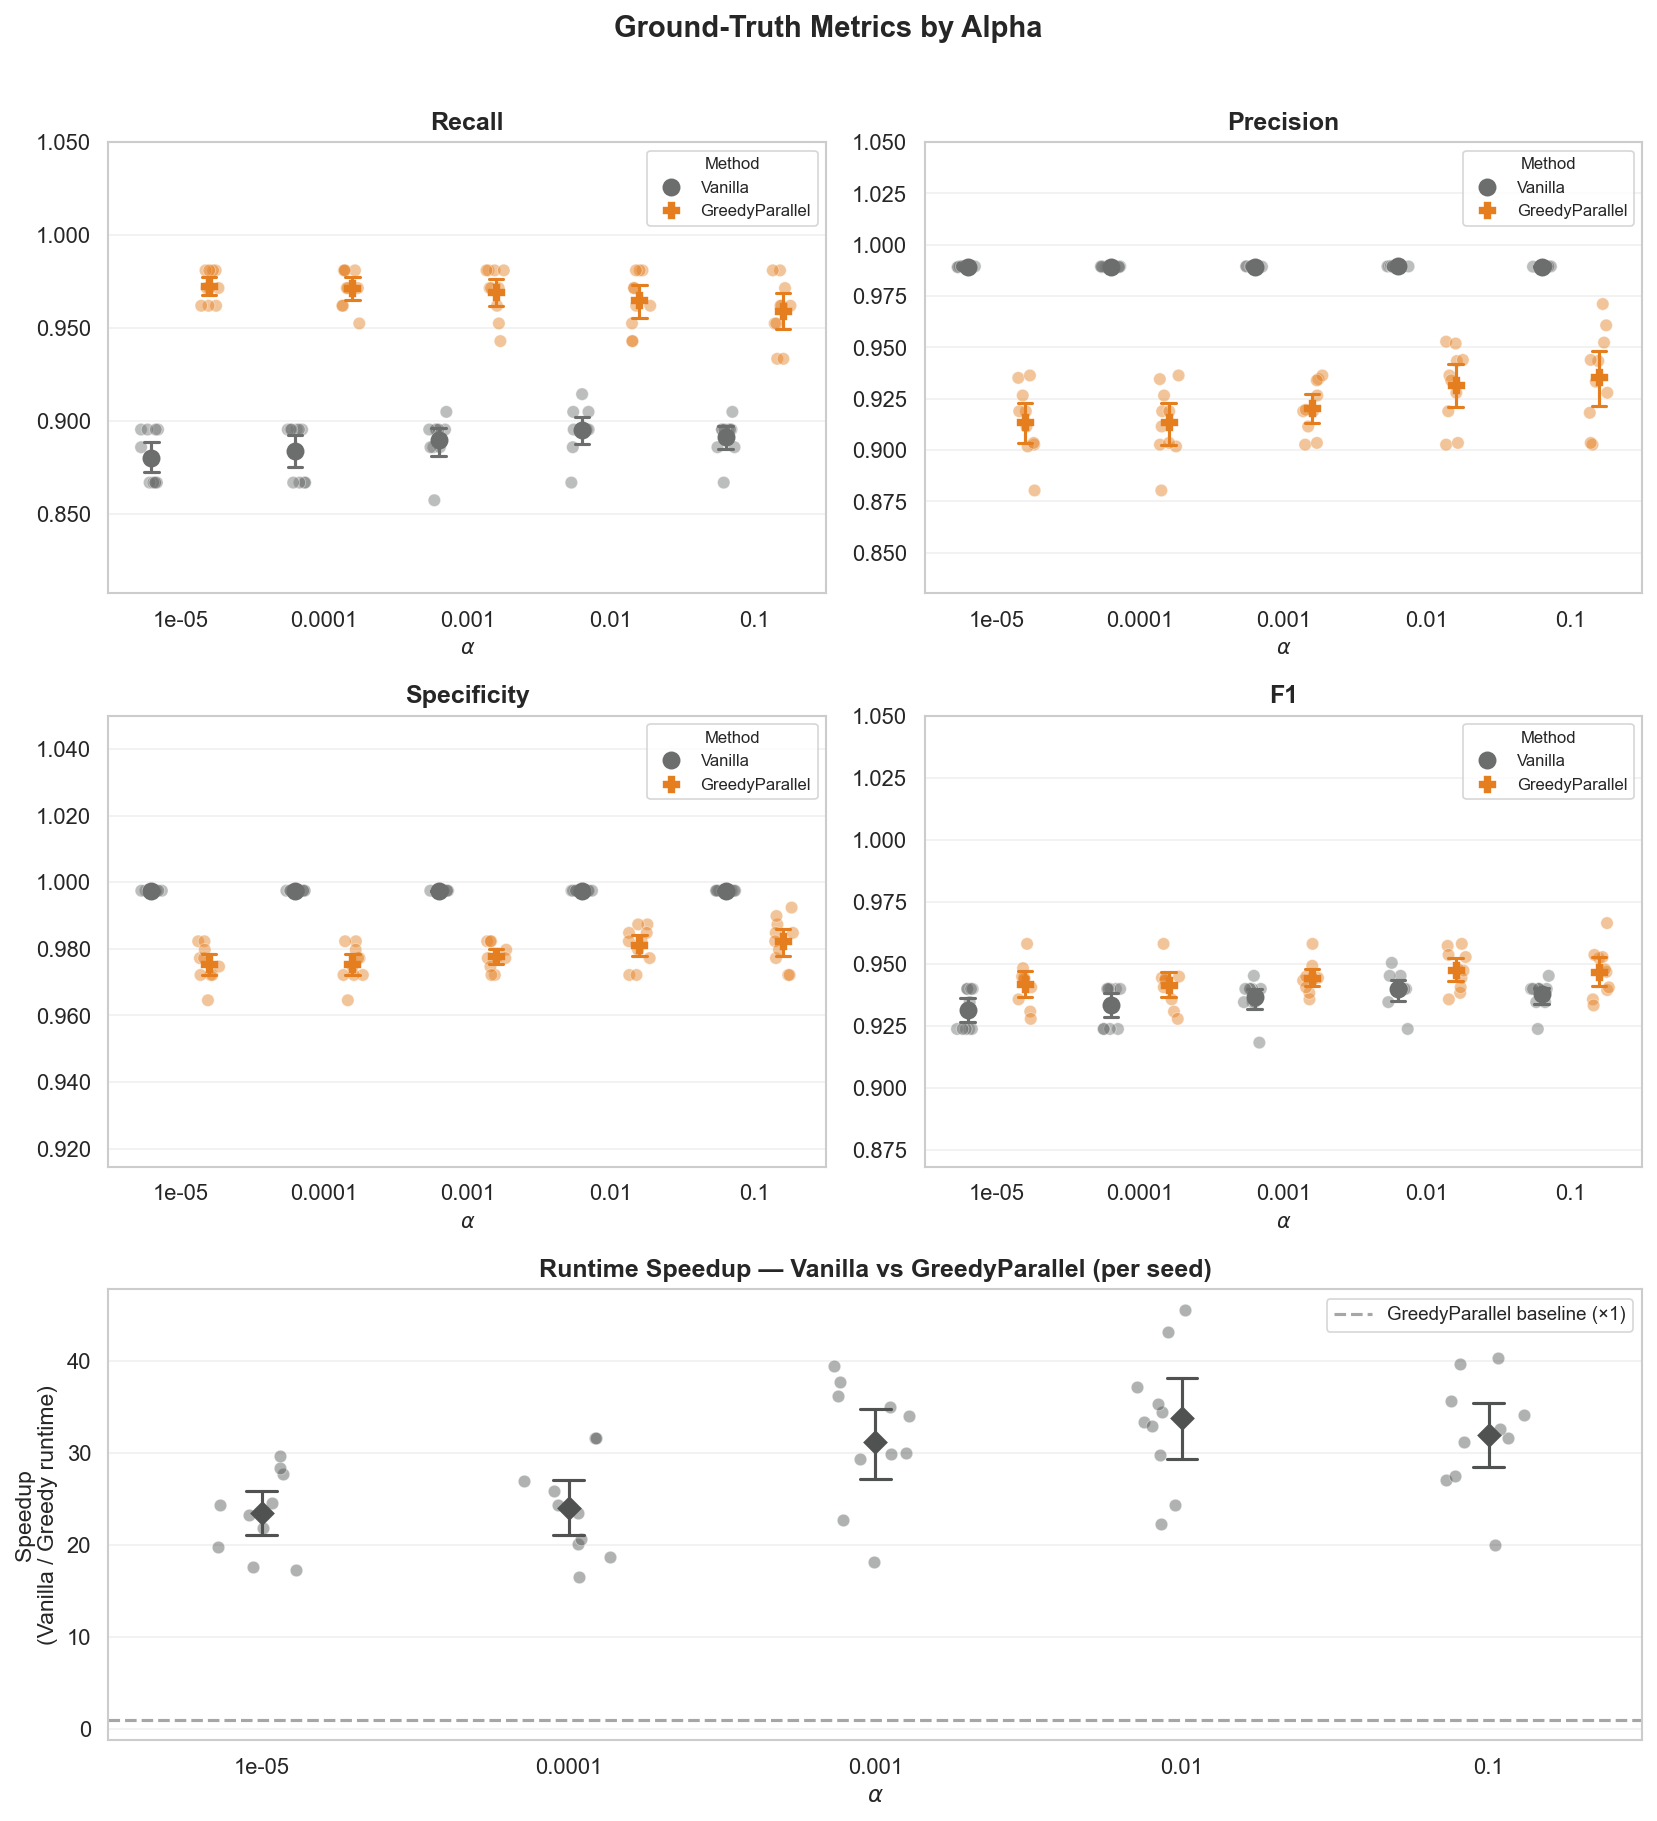
\includegraphics[width=\textwidth, height=0.8\textheight, keepaspectratio]{../benchmarks/figures/synthetic_datasets/alpha_effect_boxplots.png}
    \caption{Final-state ground-truth metrics across significance levels ($\alpha$) for Vanilla
    Boruta and Greedy Boruta on the synthetic dataset. Individual runs are shown as semi-transparent dots; markers with caps show mean $\pm$ SE.}
    \label{fig:final_state_metrics}
\end{figure}
 
Figure~\ref{fig:final_state_metrics} shows the final-state metric distributions.
Greedy Boruta achieves equal or higher Recall than Vanilla Boruta at every $\alpha$ level, in line
with Theorem~\ref{thm:recall}.
The cost is a modest reduction in Precision and Specificity: across individual runs, Greedy Boruta
incorrectly confirms between 4 and 11 noise features (out of 395), a small fraction of the
noise space.
Recall is statistically greater for Greedy Boruta (one-sided Welch $t$-test, $p < 0.01$)
and Precision and Specificity are statistically smaller at all $\alpha$ levels, as expected.
No statistically significant difference in F1 was detected between the two methods at any
$\alpha$ level (two-sided Welch $t$-test, $p > 0.01$), consistent with the competing effects
of higher recall and lower precision offsetting each other.
 
\subsubsection{Convergence and Early-Stopping Risk}
\label{sec:experiments:convergence}
 
Because Vanilla Boruta's stringent confirmation and rejection criteria often
require a large number of iterations to resolve the last few features, an
experienced practitioner may monitor progress and tune the
\texttt{max\_iter} and early-stopping parameters accordingly.
 
A more informative comparison between the two algorithms therefore evaluates
how results evolve over iterations rather than only at the final state (cf.\ Figure~\ref{fig:convergence_single_time}). To quantify the risk a practitioner faces when stopping  anilla Boruta before convergence, we introduce two metrics. The \emph{Undecidedness factor} $U = N_{\text{tentative}} / N_{\text{total}}$ measures the fraction of features that remain unresolved, and the \emph{Potential miss rate} $M = N_{\text{tentative}} / (N_{\text{tentative}} + N_{\text{confirmed}})$ measures the proportion of potentially relevant features that would be lost if all tentatives were rejected.
measures the proportion of potentially relevant features that would be lost if early stopping were triggered and all tentative features were rejected while all of them were actually relevant. Higher values of both metrics indicate greater uncertainty and risk associated with early stopping.
 
We evaluate these metrics by checkpointing Vanilla Boruta at every iteration
and tracking ground-truth metrics, using $\alpha = 0.01$.
 
\begin{figure}[H]
    \centering
    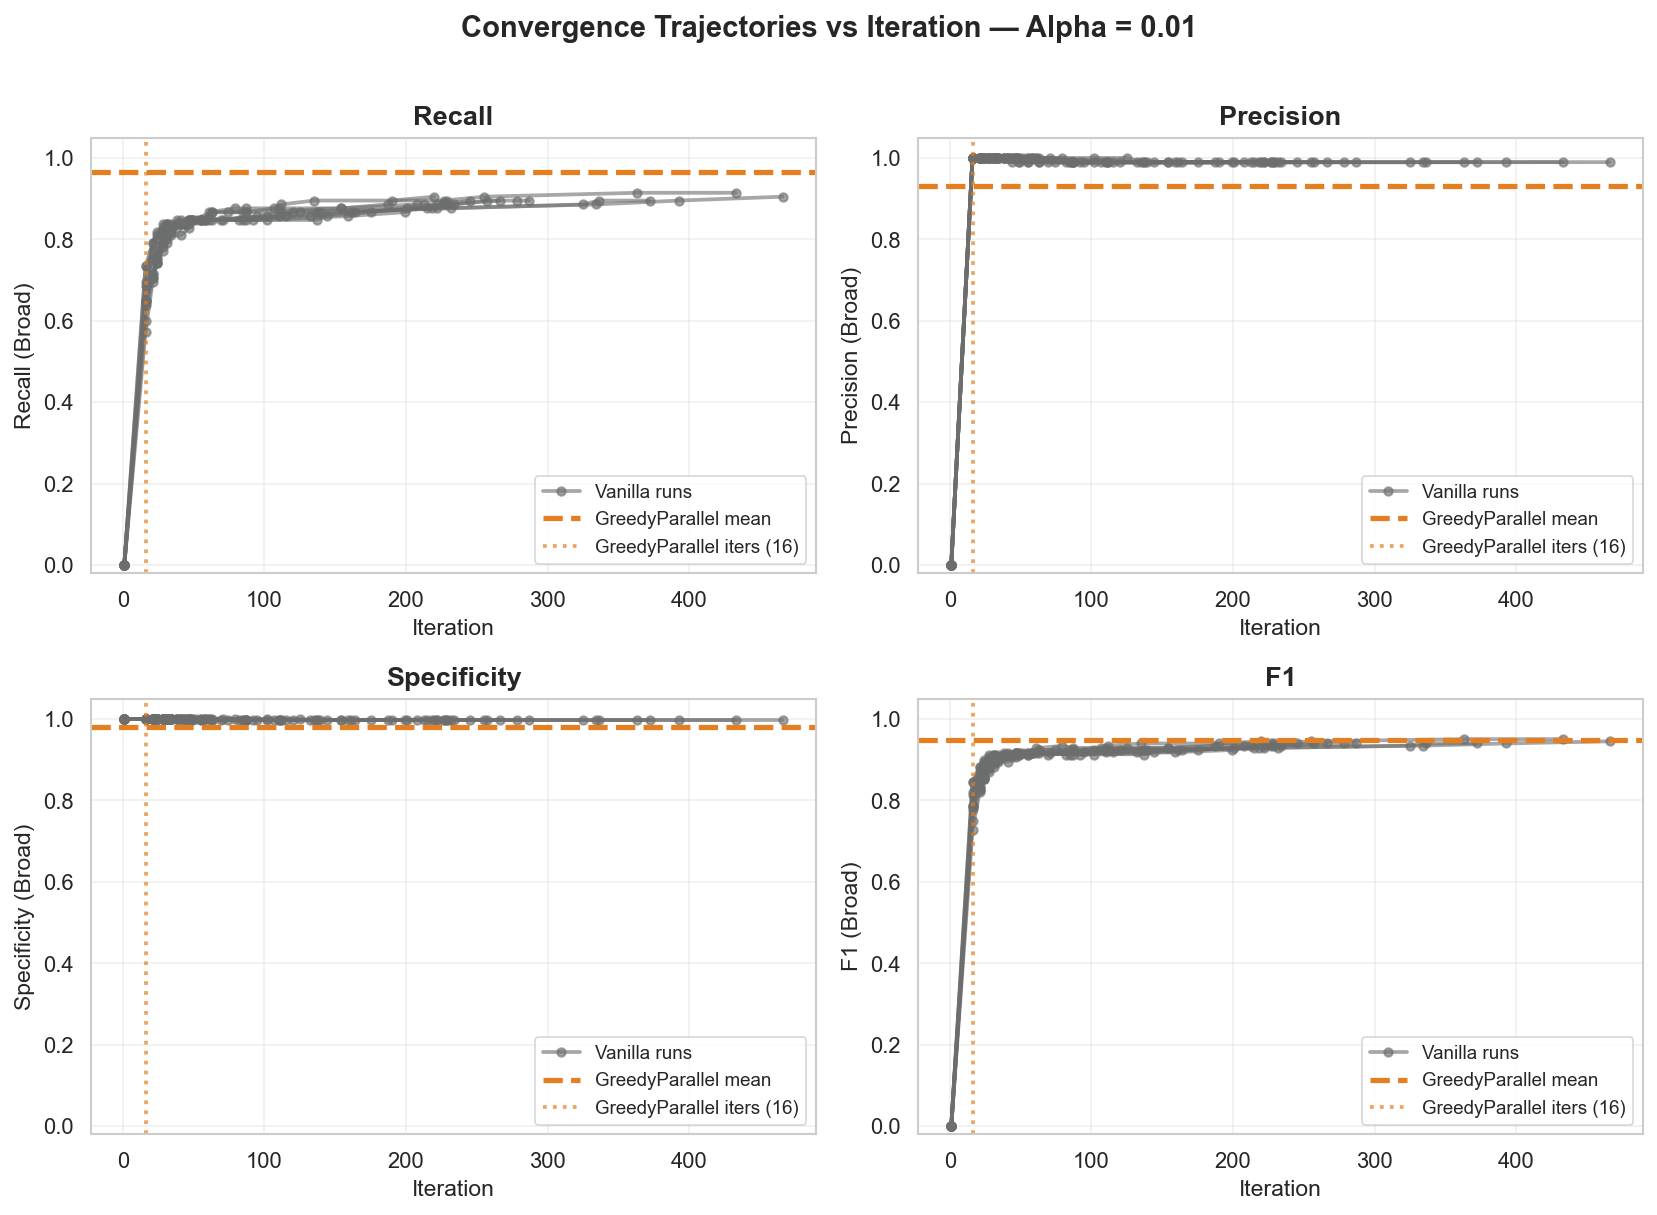
\includegraphics[width=\textwidth, height=0.45\textheight, keepaspectratio]{../benchmarks/figures/synthetic_datasets/convergence_single_alpha_iteration_0.01.png}
    \caption{Per-run convergence trajectories for $\alpha=0.01$ vs.\ iteration for all four
    GT metrics. Each grey line is one seed; the horizontal dashed line represents the Greedy Boruta mean value; The vertical dotted line marks the Greedy Boruta iteration count ($K = 16$).}
    \label{fig:convergence_single_time}
\end{figure}
 
\begin{figure}[H]
    \centering
    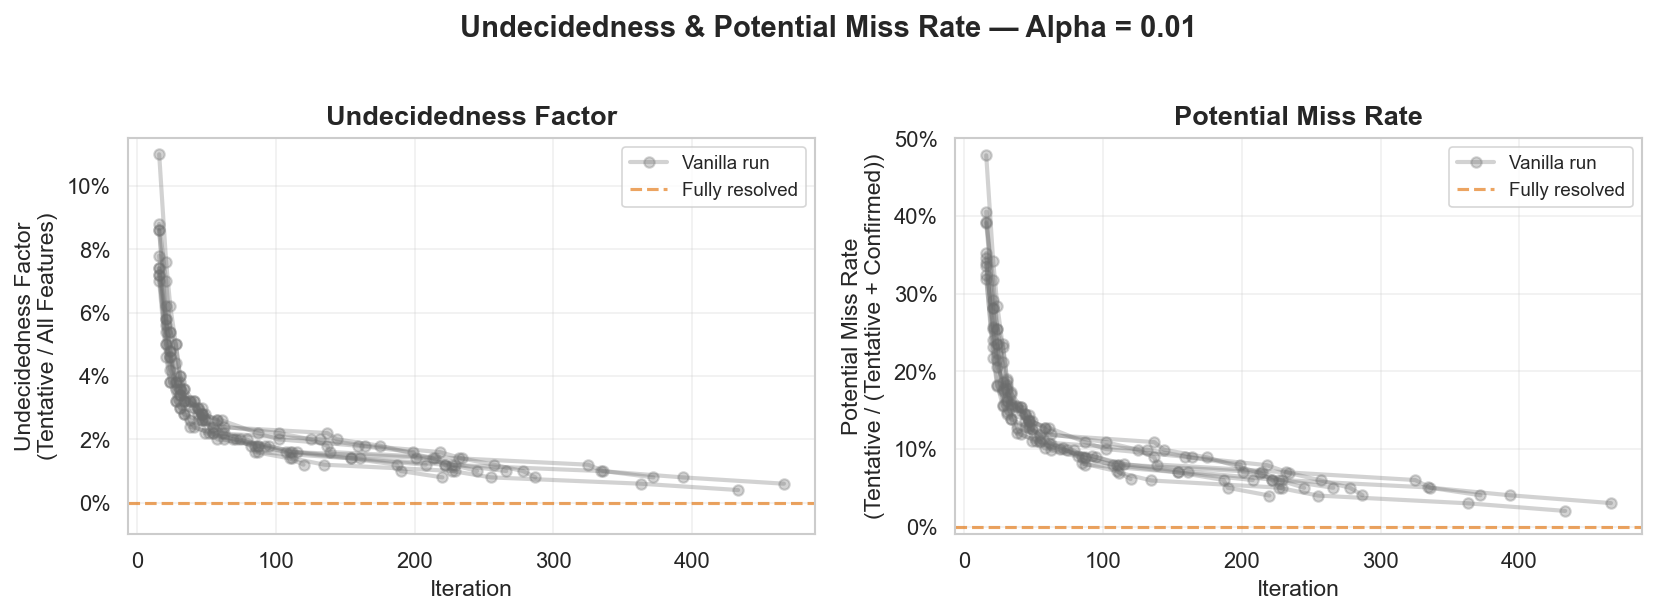
\includegraphics[width=\textwidth, height=0.38\textheight, keepaspectratio]{../benchmarks/figures/synthetic_datasets/undecidedness_single_alpha_0.01.png}
    \caption{Undecidedness factor (left) and Potential miss rate (right) for Vanilla Boruta
    at $\alpha=0.01$ as a function of iteration number. The vertical dotted line marks the
    Greedy Boruta iteration count ($K = 16$).}
    \label{fig:undecidedness_single}
\end{figure}

Figure~\ref{fig:convergence_single_time} illustrates the computational cost of determining the
final features in Vanilla Boruta. The convergence curves reveal a sharp increase in recall
during the first tenth of algorithm execution, followed by a plateau-like region where recall
improves slowly until either the early stopping criterion is triggered or the maximum number of
iterations is reached. Greedy Boruta resolves this inefficiency by confirming all features
within $K$ iterations, achieving comparable recall in substantially less time.


One might consider reducing this problem in Vanilla Boruta by lowering the maximum iteration
count or tightening early stopping parameters. However, as Figure~\ref{fig:undecidedness_single}
shows, this approach carries significant risk: prematurely terminating leaves tentative features
to be resolved entirely by the rough fix heuristic. 
% (TODO: I mean, this could be true, but even then, do the confirmed features even have formal error-rate guarantees? Under some "unreal" conditions, they do, but I think this is not why the rough fix is a problem).
Even after 100 iterations---over six times the Greedy Boruta iteration count---approximately
2\% of the initial feature set remains unresolved, and the potential miss rate is ${\sim}10\%$,
indicating that early termination would risk discarding over 10\% of features that might
eventually be confirmed as relevant.
 
\subsubsection{Runtime Speedup}
\label{sec:experiments:speedup}
 
% \begin{figure}[H]
%     \centering
%     \includegraphics[width=\textwidth, height=0.38\textheight, keepaspectratio]{../benchmarks/figures/speedup_by_alpha.png}
%     \caption{Per-seed runtime speedup (Vanilla Boruta time / Greedy Boruta time at the same seed)
%     across $\alpha$ values (log scale). The dashed horizontal line marks the Greedy Boruta
%     baseline ($1\times$). Each dot is one seed; the marker with caps shows mean $\pm$ SE.}
%     \label{fig:speedup}
% \end{figure}
 
Figure~\ref{fig:alpha_effect_boxplots} also displays per-seed speedup ratios, computed as the ratio of Vanilla
Boruta runtime to Greedy Boruta runtime for each random seed.
Greedy Boruta achieves consistent speedups of 20--45$\times$ across all five $\alpha$ values,
with mean speedups ranging from approximately $22\times$ at $\alpha=10^{-5}$ to $34\times$ at
$\alpha=10^{-2}$.
As noted in Section~\ref{sec:experiments:setup}, this speedup combines the effect of fewer
iterations (the dominant factor) with outer iteration-level parallelism (a secondary factor).
The speedup does not vary monotonically with $\alpha$ due to competing effects in the Vanilla
Boruta algorithm: at higher $\alpha$ values, the relaxed statistical testing threshold allows
Vanilla Boruta to converge more readily and terminate sooner, whereas at smaller $\alpha$ values,
the stringent confirmation and rejection criteria are so difficult to satisfy that early stopping
triggers more frequently, also shortening execution.
 
Combined with the quality results presented in Section~\ref{sec:experiments:alpha}, Greedy Boruta
delivers a 20--45$\times$ runtime reduction while achieving equal or superior Recall and
comparable F1 scores, establishing it as the preferable choice on this benchmark (TODO: is this last statement "too bold" for a scientific paper?).

% =============================================================================
% SECTION 5.3 — REAL-WORLD BENCHMARKS (draft)
% =============================================================================
% NOTES FOR NICOLAS:
%   - SE values marked [SE] need to be filled from experimental data
%   - Dexter vs. Dorothea: currently using Dexter (matches stats/plots).
%     Check whether Dorothea should also be included or replaces Dexter.
%   - Image paths assume ../benchmarks/figures/; adjust as needed.
%   - Vanilla (Soft/All) variant dropped per decision; only Strict used.
%   - riboflavin is regression (R²); all others are classification (F1).
% =============================================================================
 
\subsection{Real-World Benchmarks}
\label{sec:experiments:realworld}
 
To validate Greedy Boruta beyond controlled synthetic settings, we evaluate on six
publicly available high-dimensional benchmarks spanning classification and regression
tasks (Table~\ref{tab:realworld_datasets}).
Because ground-truth relevant feature sets are not available for these datasets,
we assess selection quality indirectly: both methods select features independently,
a downstream model (Light Gradient Boosting Method \cite{ke2017lightgbm}) is trained on the selected subset, and performance is measured on using cross-validation (5 folds) and weighted F1 (classification) or~$R^2$ (regression).
Each (dataset, $\alpha$, method) configuration is repeated over $R = 10$ independent
random seeds; results are reported as mean~$\pm$~SE.
 
\begin{table}[H]
\centering
\caption{Real-world benchmark datasets.}
\label{tab:realworld_datasets}
\begin{tabular}{llrrll}
\toprule
Dataset    & Domain          & $n$    & $p$      & Task           & Source \\
\midrule
% Madelon    & Artificial      & 2{,}000  & 500    & Classification & NIPS 2003 \\
% Gisette    & Digit recog.    & 6{,}000  & 5{,}000  & Classification & NIPS 2003 \\
% Arcene     & Mass spectrom.  & 100    & 10{,}000 & Classification & NIPS 2003 \\
% Dexter     & Text classif.   & 300    & 20{,}000 & Classification & NIPS 2003 \\
% Isolet     & Speech recog.   & 7{,}797  & 617    & Classification & UCI \\
% Riboflavin & Gene expression & 71     & 4{,}088  & Regression     & \addcite{R package hdi} \\
Madelon    & Artificial      & 2{,}000  & 500      & Classification & \cite{guyon2004result} \\
Gisette    & Digit recog.    & 6{,}000  & 5{,}000  & Classification & \cite{guyon2004result} \\
Arcene     & Mass spectrom.  & 100      & 10{,}000 & Classification & \cite{guyon2004result} \\
Dexter     & Text classif.   & 300      & 20{,}000 & Classification & \cite{guyon2004result} \\
Isolet     & Speech recog.   & 7{,}797  & 617      & Classification & \cite{uci2017} \\
Riboflavin & Gene expression & 71       & 4{,}088  & Regression     & \cite{buhlmann2014hdi} \\
\bottomrule
\end{tabular}
\end{table}

 
The significance level is swept over $\alpha \in \{10^{-1},\, 10^{-3},\, 10^{-5}\}$, a reduced set, since  these experiments are much more computationally intensive. All other experimental settings (base estimator, parallelism configuration, hardware) are identical to those described in Section~\ref{sec:experiments:setup}. Vanilla Boruta is compared using the \emph{strict} feature set, i.e., only features confirmed by the binomial test or the rough fix heuristic, excluding tentative features (TODO: is this true? Verify).
 
% -----------------------------------------------------------------------------
\subsubsection{Downstream Performance}
\label{sec:experiments:realworld:performance}
 
Table~\ref{tab:realworld_results} presents the downstream performance, runtime, and
speedup for each dataset and significance level.
To assess whether the observed performance differences are statistically meaningful,
we conduct one-sided Welch $t$-tests at significance level $0.01$: one testing
whether Greedy Boruta is significantly better, and the converse.
The ``Sig.'' column reports the outcome: $\approx$ indicates no statistically
significant difference (tie), $\blacktriangleright$ indicates Vanilla is significantly
better, and $\blacktriangleleft$ indicates Greedy is significantly better.
 
% \begin{table}[H]
% \caption{Real-world benchmark results (mean $\pm$ SE over 5 seeds).
% Score is weighted F1 for classification tasks and $R^2$ for Riboflavin.
% Sig.\ column: $\approx$ = no significant difference;
% $\blacktriangleright$ = Vanilla significantly better;
% $\blacktriangleleft$ = Greedy significantly better
% (one-sided Welch $t$-test, $p < 0.05$).}
% \label{tab:realworld_results}
% \centering
% \small
% \begin{tabular}{ll rr rr c r}
% \toprule
% & & \multicolumn{2}{c}{Greedy Boruta}
% & \multicolumn{2}{c}{Vanilla Boruta} & & \\
% \cmidrule(lr){3-4} \cmidrule(lr){5-6}
% Dataset & $\alpha$ & Score & Time (s)
%                    & Score & Time (s)
%                    & Sig. & Speedup \\
% \midrule
% \multirow{3}{*}{Madelon}
%   & $10^{-1}$  & $.855 \pm 0.001 \text{\scriptsize[SE]}$ & --
%                & $.862 \pm 0.002 \text{\scriptsize[SE]}$ & --
%                & $\blacktriangleright$ & $14.6\times$ \\
%   & $10^{-3}$  & $.856 \pm \text{\scriptsize[SE]}$ & --
%                & $.866 \pm \text{\scriptsize[SE]}$ & --
%                & $\blacktriangleright$ & $10.8\times$ \\
%   & $10^{-5}$  & $.855 \pm \text{\scriptsize[SE]}$ & --
%                & $.866 \pm \text{\scriptsize[SE]}$ & --
%                & $\blacktriangleright$ & $9.5\times$ \\
% \midrule
% \multirow{3}{*}{Arcene}
%   & $10^{-1}$  & $.868 \pm \text{\scriptsize[SE]}$ & --
%                & $.878 \pm \text{\scriptsize[SE]}$ & --
%                & $\approx$ & $16.3\times$ \\
%   & $10^{-3}$  & $.874 \pm \text{\scriptsize[SE]}$ & --
%                & $.878 \pm \text{\scriptsize[SE]}$ & --
%                & $\approx$ & $14.5\times$ \\
%   & $10^{-5}$  & $.874 \pm \text{\scriptsize[SE]}$ & --
%                & $.877 \pm \text{\scriptsize[SE]}$ & --
%                & $\approx$ & $10.8\times$ \\
% \midrule
% \multirow{3}{*}{Gisette}
%   & $10^{-1}$  & $.982 \pm \text{\scriptsize[SE]}$ & --
%                & $.982 \pm \text{\scriptsize[SE]}$ & --
%                & $\approx$ & $22.9\times$ \\
%   & $10^{-3}$  & $.982 \pm \text{\scriptsize[SE]}$ & --
%                & $.983 \pm \text{\scriptsize[SE]}$ & --
%                & $\approx$ & $16.0\times$ \\
%   & $10^{-5}$  & $.982 \pm \text{\scriptsize[SE]}$ & --
%                & $.982 \pm \text{\scriptsize[SE]}$ & --
%                & $\approx$ & $13.4\times$ \\
% \midrule
% \multirow{3}{*}{Dexter}
%   & $10^{-1}$  & $.935 \pm \text{\scriptsize[SE]}$ & --
%                & $.934 \pm \text{\scriptsize[SE]}$ & --
%                & $\approx$ & $7.9\times$ \\
%   & $10^{-3}$  & $.936 \pm \text{\scriptsize[SE]}$ & --
%                & $.935 \pm \text{\scriptsize[SE]}$ & --
%                & $\approx$ & $6.3\times$ \\
%   & $10^{-5}$  & $.936 \pm \text{\scriptsize[SE]}$ & --
%                & $.935 \pm \text{\scriptsize[SE]}$ & --
%                & $\approx$ & $6.2\times$ \\
% \midrule
% \multirow{3}{*}{Riboflavin}
%   & $10^{-1}$  & $.580 \pm \text{\scriptsize[SE]}$ & --
%                & $.539 \pm \text{\scriptsize[SE]}$ & --
%                & $\approx$ & $2.1\times$ \\
%   & $10^{-3}$  & $.583 \pm \text{\scriptsize[SE]}$ & --
%                & $.541 \pm \text{\scriptsize[SE]}$ & --
%                & $\approx$ & $1.9\times$ \\
%   & $10^{-5}$  & $.582 \pm \text{\scriptsize[SE]}$ & --
%                & $.544 \pm \text{\scriptsize[SE]}$ & --
%                & $\approx$ & $1.7\times$ \\
% \midrule
% \multirow{3}{*}{Isolet}
%   & $10^{-1}$  & $.958\pm \text{\scriptsize[SE]}$ & --
%                & $.959 \pm \text{\scriptsize[SE]}$ & --
%                & $\approx$ & $66.2\times$ \\
%   & $10^{-3}$  & $.959 \pm \text{\scriptsize[SE]}$ & --
%                & $.959 \pm \text{\scriptsize[SE]}$ & --
%                & $\approx$ & $48.7\times$ \\
%   & $10^{-5}$  & $.959 \pm \text{\scriptsize[SE]}$ & --
%                & $.958 \pm \text{\scriptsize[SE]}$ & --
%                & $\approx$ & $42.4\times$ \\
% \bottomrule
% \end{tabular}
% \end{table}

\begin{table}[H]
\caption{Real-world benchmark results (mean $\pm$ SE over $R=10$ seeds).
\emph{Score} is test-set F1 (classification) or $R^2$ (regression).
\emph{Sig.}:\ directional one-sided Welch $t$-test at level $0.01$;
$\blacktriangleright$~= Vanilla significantly better,
$\blacktriangleleft$~= Greedy significantly better,
$\approx$~= no significant difference.
\emph{Speedup} = Vanilla time\,/\,Greedy time.}
\label{tab:realworld_results}
\centering
\small
\begin{tabular}{ll cc cc c r}
\toprule
& & \multicolumn{2}{c}{Greedy Boruta}
& \multicolumn{2}{c}{Vanilla Boruta} & & \\
\cmidrule(lr){3-4} \cmidrule(lr){5-6}
Dataset & $\alpha$ & Score & Time (s)
                   & Score & Time (s)
                   & Sig. & Speedup \\
\midrule
\multirow{3}{*}{Madelon}
  & $10^{-1}$  & $.856 \pm .002$ & 2.4
               & $.862 \pm .002$ & 34.7
               & $\blacktriangleright$ & $14.6\times$ \\
  & $10^{-3}$  & $.856 \pm .002$ & 3.2
               & $.866 \pm .001$ & 34.8
               & $\blacktriangleright$ & $10.9\times$ \\
  & $10^{-5}$  & $.855 \pm .002$ & 4.1
               & $.866 \pm .001$ & 39.1
               & $\blacktriangleright$ & $9.5\times$ \\
\midrule
\multirow{3}{*}{Arcene}
  & $10^{-1}$  & $.868 \pm .005$ & 11.2
               & $.878 \pm .004$ & 184.3
               & $\approx$ & $16.4\times$ \\
  & $10^{-3}$  & $.875 \pm .005$ & 14.0
               & $.879 \pm .003$ & 203.3
               & $\approx$ & $14.6\times$ \\
  & $10^{-5}$  & $.875 \pm .006$ & 19.9
               & $.878 \pm .005$ & 215.7
               & $\approx$ & $10.9\times$ \\
\midrule
\multirow{3}{*}{Gisette}
  & $10^{-1}$  & $.982 \pm .0003$ & 35.4
               & $.982 \pm .0003$ & 814.0
               & $\approx$ & $23.0\times$ \\
  & $10^{-3}$  & $.982 \pm .0002$ & 49.8
               & $.983 \pm .0001$ & 801.3
               & $\approx$ & $16.1\times$ \\
  & $10^{-5}$  & $.982 \pm .0002$ & 61.5
               & $.982 \pm .0002$ & 824.1
               & $\approx$ & $13.4\times$ \\
\midrule
\multirow{3}{*}{Dexter}
  & $10^{-1}$  & $.935 \pm .002$ & 21.0
               & $.934 \pm .002$ & 165.6
               & $\approx$ & $7.9\times$ \\
  & $10^{-3}$  & $.936 \pm .002$ & 29.2
               & $.936 \pm .002$ & 185.6
               & $\approx$ & $6.4\times$ \\
  & $10^{-5}$  & $.937 \pm .002$ & 34.1
               & $.936 \pm .002$ & 212.9
               & $\approx$ & $6.2\times$ \\
\midrule
\multirow{3}{*}{Riboflavin}
  & $10^{-1}$  & $.581 \pm .019$ & 47.6
               & $.539 \pm .020$ & 100.6
               & $\approx$ & $2.1\times$ \\
  & $10^{-3}$  & $.584 \pm .017$ & 64.6
               & $.542 \pm .021$ & 125.9
               & $\approx$ & $1.9\times$ \\
  & $10^{-5}$  & $.583 \pm .017$ & 86.8
               & $.545 \pm .021$ & 154.5
               & $\approx$ & $1.8\times$ \\
\midrule
\multirow{3}{*}{Isolet}
  & $10^{-1}$  & $.959 \pm .0003$ & 5.1
               & $.959 \pm .0002$ & 340.2
               & $\approx$ & $66.2\times$ \\
  & $10^{-3}$  & $.959 \pm .0003$ & 7.3
               & $.959 \pm .0003$ & 355.0
               & $\approx$ & $48.8\times$ \\
  & $10^{-5}$  & $.959 \pm .0003$ & 9.3
               & $.958 \pm .0002$ & 393.6
               & $\approx$ & $42.5\times$ \\
\bottomrule
\end{tabular}
\end{table}
 
Of the 18 (dataset, $\alpha$) configurations, 15 show no statistically significant difference in downstream performance between the two methods. In 3 configurations (Madelon at all three $\alpha$ levels), Vanilla Boruta achieves a statistically significant but practically small advantage: the largest observed gap is ${\sim}0.01$ in F1 (Madelon, $\alpha = 10^{-5}$).

Importantly, these performance differences, whether favourable or unfavourable to Greedy Boruta, are negligible in absolute terms, while the runtime reductions are substantial. Speedups range from $2.2\times$ (Riboflavin, $\alpha = 10^{-5}$) to $66.2\times$ (Isolet, $\alpha = 0.1$), 
with larger speedups observed on datasets where Vanilla Boruta requires more iterations to resolve features, which depends on the signal-to-noise characteristics of the data rather than dimensionality alone. (TODO: should we include this comment? Is this true?). 

Figure~\ref{fig:realworld_boxplots} shows the full score distributions
across seeds, confirming that the inter-method differences are small relative
to the run-to-run variability within each method.
 
\begin{figure}[H]
    \centering
    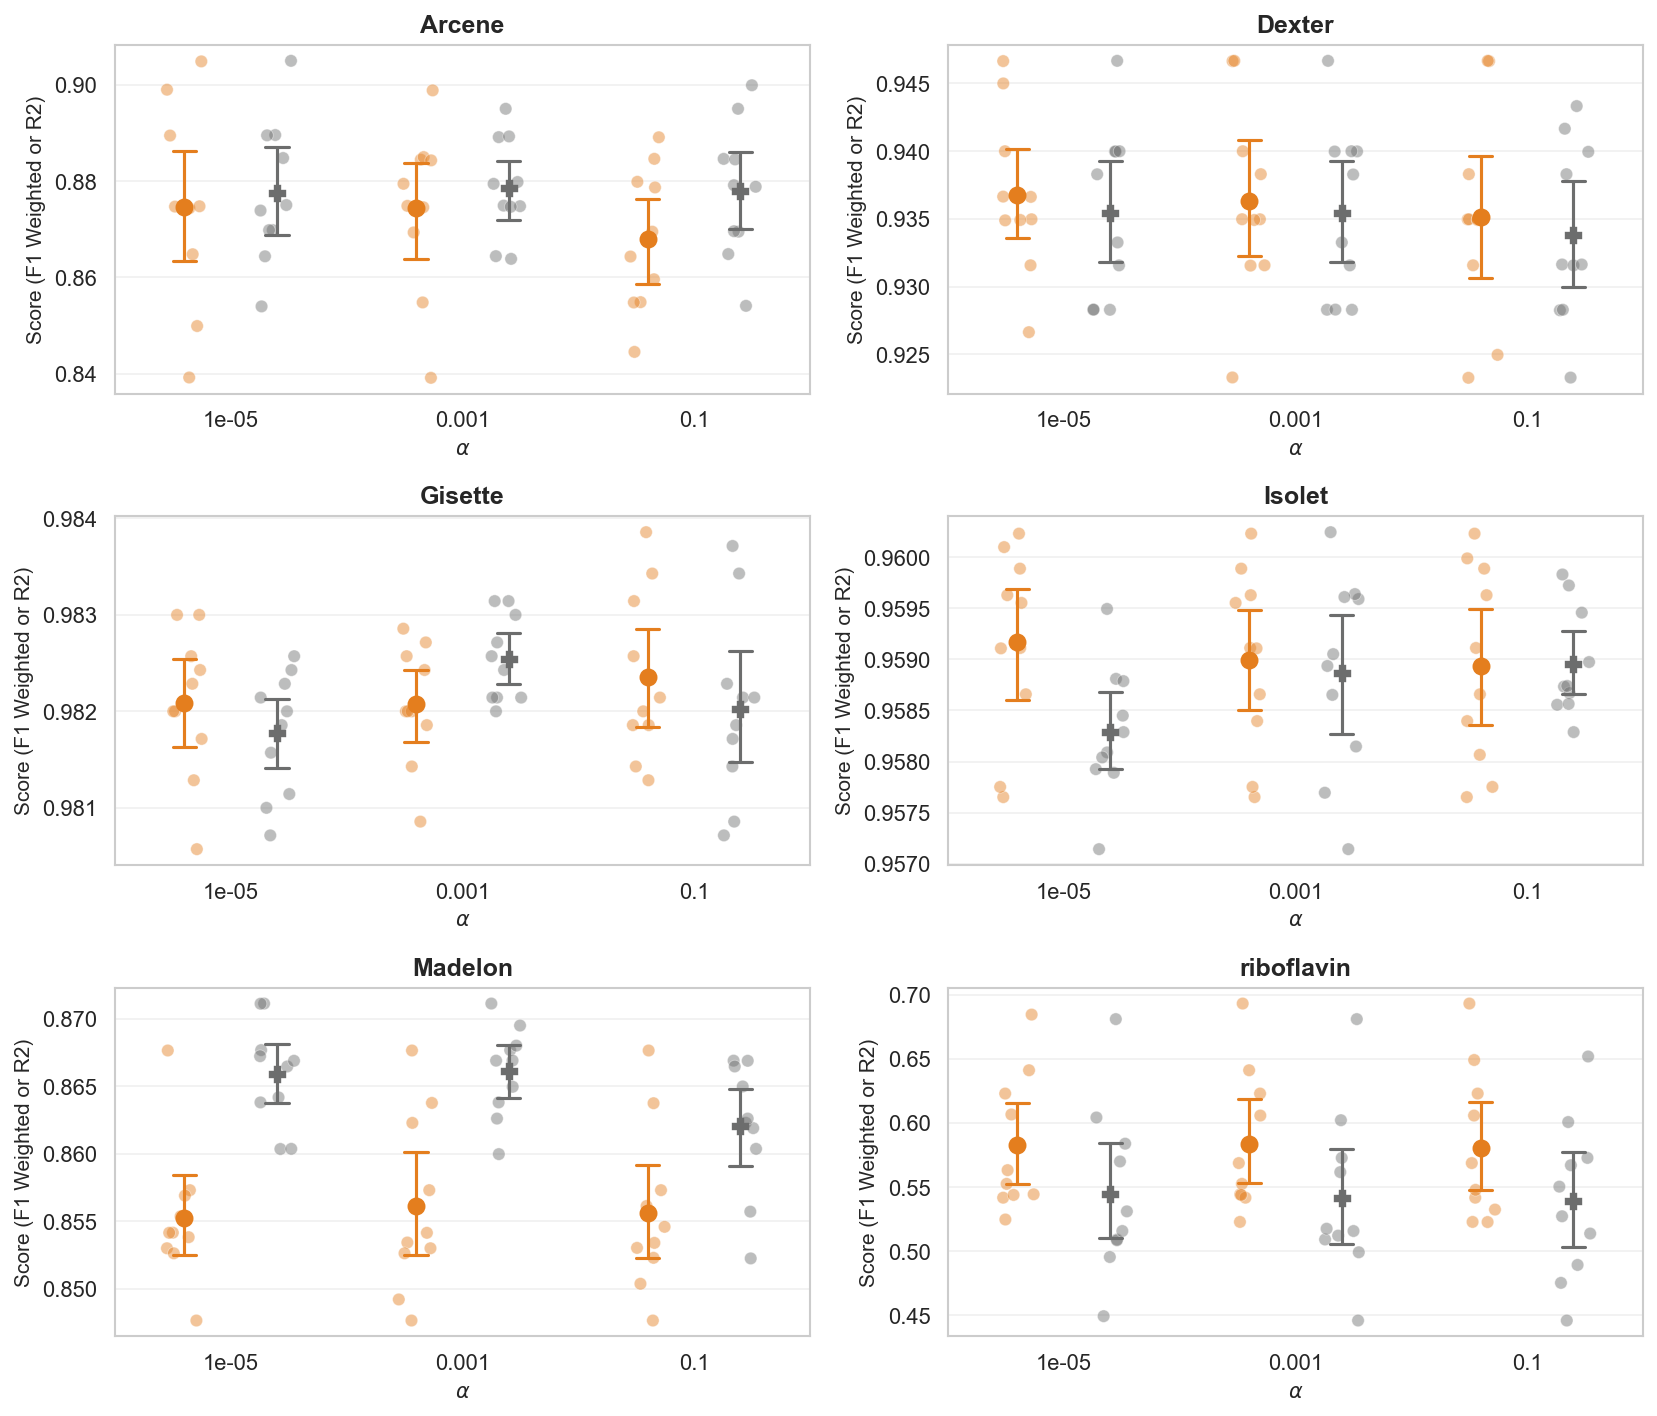
\includegraphics[width=\textwidth, height=1\textheight, keepaspectratio]{../benchmarks/figures/real_datasets/score_comparison.png}
    \caption{Downstream performance (weighted F1 or $R^2$) across significance
    levels for each dataset (5 seeds per configuration). The narrow interquartile
    ranges and overlapping boxes confirm that performance differences between
    methods are small relative to run-to-run variability.}
    \label{fig:realworld_boxplots}
\end{figure}
 
% -----------------------------------------------------------------------------
\subsubsection{Pareto Efficiency: Performance vs.\ Cost}
\label{sec:experiments:realworld:pareto}
 
To visualise the performance--cost trade-off across all datasets simultaneously,
Figure~\ref{fig:pareto} plots the mean downstream score against mean wall-clock
time for each (dataset, $\alpha$, method) configuration.
Points sharing the same colour represent the same dataset; circles denote
Greedy Boruta and crosses denote Vanilla Boruta; within each (dataset, method)
group, the different points correspond to different $\alpha$ values.
 
\begin{figure}[H]
    \centering
    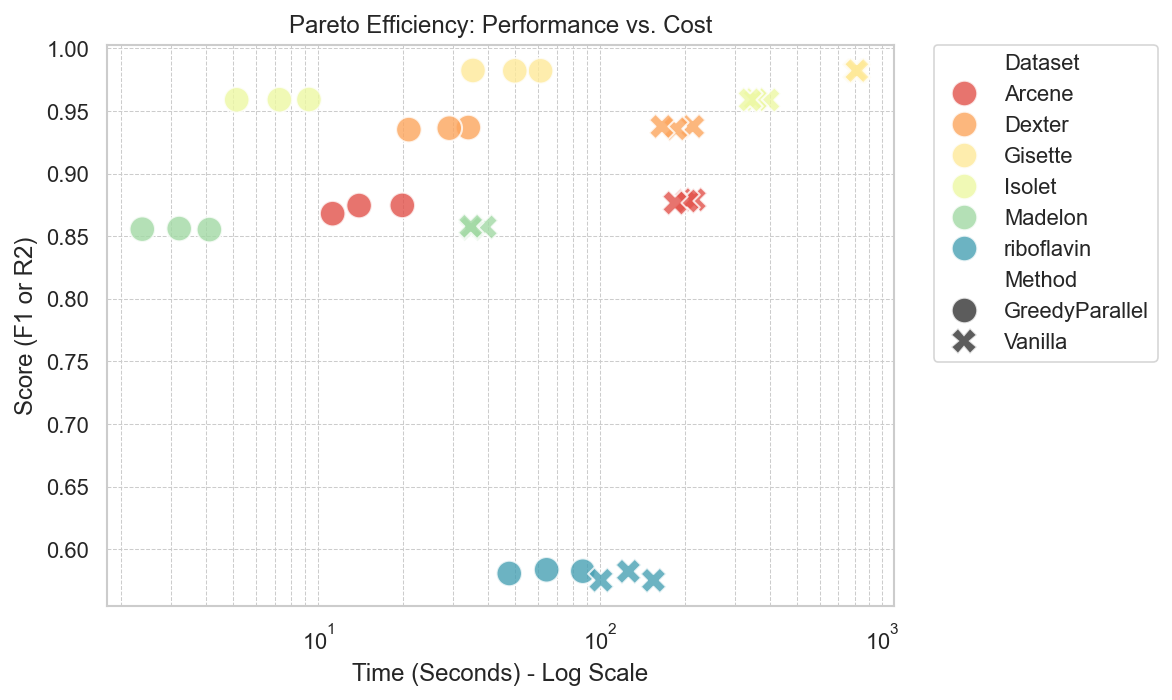
\includegraphics[width=\textwidth, height=0.42\textheight, keepaspectratio]{../benchmarks/figures/real_datasets/pareto_efficiency.png}
    \caption{Pareto efficiency plot: downstream score vs.\ wall-clock time (log scale)
    for all (dataset, $\alpha$, method) configurations.
    Each colour represents a dataset; circles are Greedy Boruta, crosses are
    Vanilla Boruta.
    Points of the same colour and marker correspond to different $\alpha$ levels.
    Greedy Boruta consistently occupies the upper-left region (high performance,
    low cost), Pareto-dominating or matching Vanilla Boruta on every dataset.}
    \label{fig:pareto}
\end{figure}
 
% The plot reveals a striking pattern (TODO: stereotypical AI writing feature change/remove the start of the paragraph + too informal for a scientific paper): for every dataset, 
Across all six datasets, the Greedy Boruta points (circles) sit at or near the same vertical position as the corresponding Vanilla Boruta points (crosses) but are displaced one to two orders of magnitude to the left on the time axis. This means Greedy Boruta achieves equivalent downstream performance at a fraction of the computational cost, Pareto-dominating Vanilla Boruta in the majority of configurations.

% The only dataset where Vanilla points sit consistently (though slightly) above the Greedy points is Madelon , consistent with the statistical tests in Table~\ref{tab:realworld_results}; even there, the vertical gap is small (${\sim}0.005$--$0.01$ in F1) while the horizontal gap spans an order of magnitude in runtime (TODO: Not really, Madelon is kinda indistinguishable, but on arcene we can see the points slightly above on vanilla. I will run 10 seeds to see if the results are statistically significant).
 
For the practitioner, this plot encapsulates the central practical claim of this paper: Greedy Boruta offers an almost strictly better trade-off between selection quality and computational cost across a wide range of dataset characteristics and significance levels.
 
% -----------------------------------------------------------------------------
\subsubsection{Convergence on Real Data}
\label{sec:experiments:realworld:convergence}
 
% The convergence difficulties documented for the synthetic benchmark in Section~\ref{sec:experiments:convergence} are not an artefact of the controlled setting---they persist on real-world data (TODO: Do we need this "intro" the convergence plots? Perhaps simplify).
% To illustrate this, we checkpoint Vanilla Boruta at every iteration on the Gisette
% dataset ($p = 5{,}000$) and track the undecidedness factor and potential miss rate
% across three significance levels.

We repeat the convergence analysis from Section~\ref{sec:experiments:convergence} on real data by checkpointing Vanilla Boruta at every iteration on Gisette ($p = 5{,}000$) with $\alpha = 0.1$.

\begin{figure}[H]
    \centering
    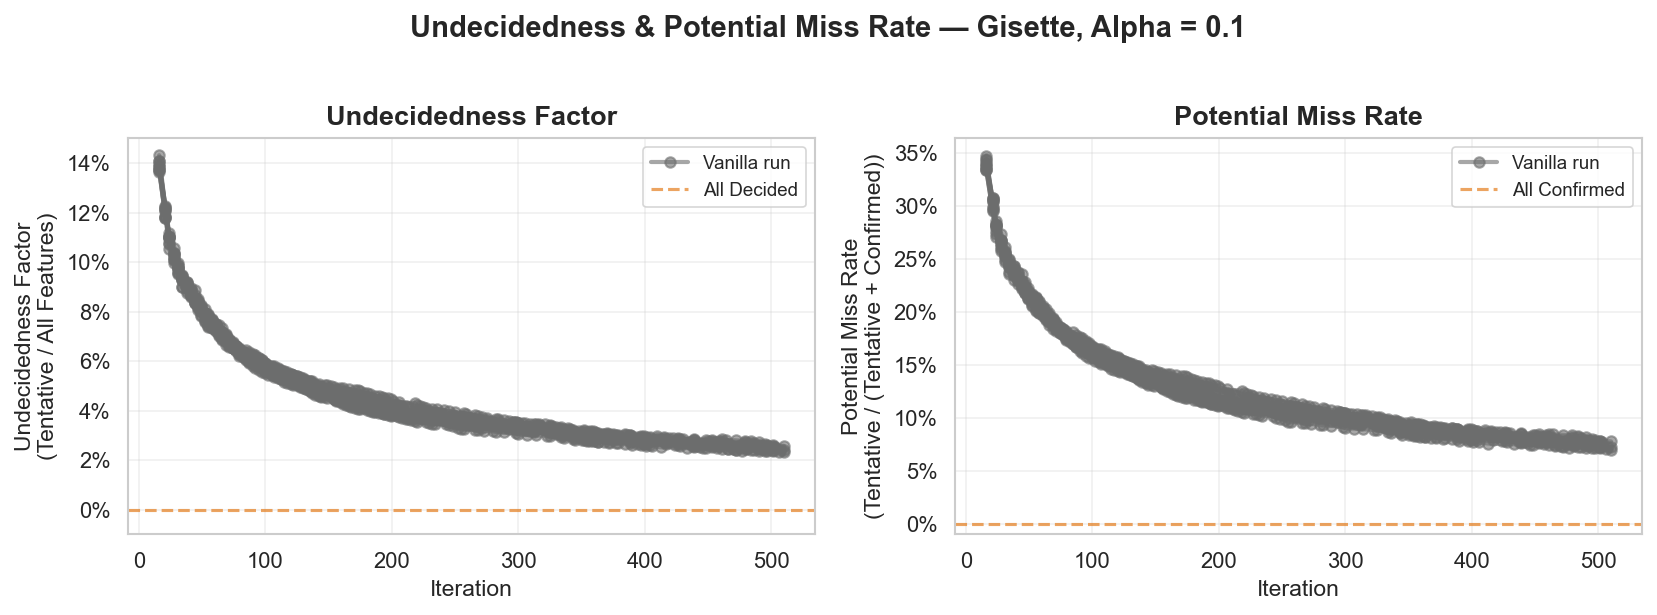
\includegraphics[width=\textwidth, height=0.28\textheight, keepaspectratio]{../benchmarks/figures/real_datasets/undecidedness_single_alpha_Gisette_0.1.png}
    \caption{Left: Undecidedness factor
    for Vanilla Boruta on Gisette with $\alpha = \{10^{-1}\}$
    as a function of iteration number .
    Right: Potential miss rate for Vanilla Boruta on Gisette with $\alpha = \{10^{-1}\}$, as a function of iteration number.
    10 seeds per panel. The dashed lines marks complete resolution (0\%).}
    \label{fig:undecidedness_miss_rate_gisette}
\end{figure}

% \begin{figure}[H]
%     \centering
%     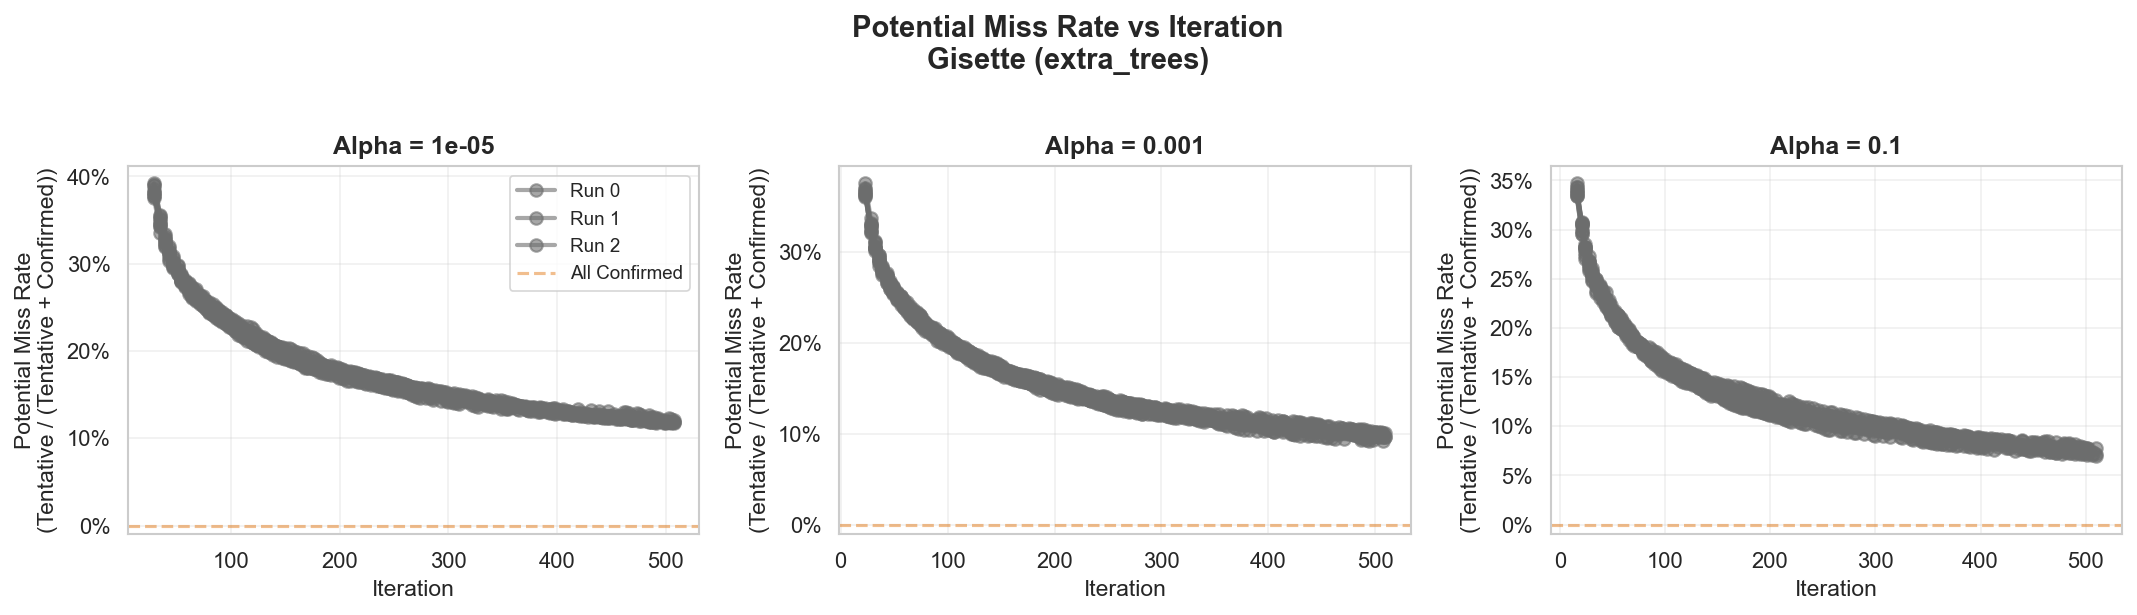
\includegraphics[width=\textwidth, height=0.28\textheight, keepaspectratio]{../benchmarks/figures/real_datasets/potential_miss_rate_iteration_Gisette.png}
%     \caption{Potential miss rate (fraction of tentative features among all
%     potentially relevant features) for Vanilla Boruta on Gisette vs.\ wall-clock
%     time (3 seeds per panel).
%     At the 512-iteration budget, approximately 5--11\% of potentially relevant
%     features remain unresolved, depending on $\alpha$.}
%     \label{fig:miss_rate_gisette}
% \end{figure}

Figure~\ref{fig:undecidedness_miss_rate_gisette} shows that the undecidedness factor
follows the same characteristic decay observed on synthetic data: a rapid
initial drop as clearly informative and clearly irrelevant features are
resolved, followed by a long tail where the remaining borderline features
resist classification.
After the full 512-iteration budget, 2--3\% of Gisette's 5{,}000 features
remain tentative across all $\alpha$ levels and seeds---corresponding to
100--200 features whose status is ultimately resolved by the rough fix
heuristic rather than the principled binomial test.
 
Figure~\ref{fig:undecidedness_miss_rate_gisette} translates this into practical risk:
the potential miss rate, which measures the fraction of possibly relevant
features that would be lost if tentatives were discarded, plateaus at
approximately 6\% with $\alpha = 0.1$, which is a lenient configuration for Vanilla Boruta.
% This confirms that the convergence problem is not merely academic (TODO: stereotypical AI writing feature change/remove the start of the paragraph + too informal for a scientific paper), on a real high-dimensional dataset, a practitioner stopping Vanilla Boruta early (or at the default iteration budget) faces meaningful uncertainty about whether the selected feature set is complete.
On this real high-dimensional dataset, a practitioner stopping Vanilla Boruta early faces  uncertainty about whether the selected feature set is complete.
Greedy Boruta eliminates this uncertainty entirely: on Gisette with
$\alpha = 0.1$, convergence requires $K = \lceil \log_2(5000/0.1)
\rceil = 16$ iterations, resolving all 5{,}000 features with no tentatives
and no reliance on heuristic post-processing.
 
% \decision{Move Gisette convergence plots to supplementary and show only a summary sentence here? Or keep in main body? Depends on final page count. Equivalent plots for other datasets can go in an appendix.}

% -----------------------------------------------------------------------------
\subsubsection{Summary}
\label{sec:experiments:realworld:summary}
 
The real-world benchmarks reinforce the conclusions from the synthetic experiments. Greedy Boruta delivers speedups of $2\times$--$66\times$ across six datasets spanning $p = 500$ to $p = 20{,}000$ features, with downstream model performance that is statistically indistinguishable from Vanilla Boruta in 15 of 18 configurations and practically equivalent in the remaining cases (maximum gap ${\sim}0.01$ in F1 or $R^2$). 
% The convergence analysis on Gisette confirms that the tentative-feature problem is a real concern in practice, not merely a theoretical inconvenience (TODO: stereotypical AI writing feature, change).
The convergence analysis on Gisette shows that the tentative-feature problem persists on real data with practical consequences.
Together with the Pareto efficiency analysis, these results establish Greedy Boruta as the preferred method when the all-relevant paradigm is appropriate and downstream filtering is available.

% % =============================================================================
% % 6. DISCUSSION (~0.75 page)
% % =============================================================================
% \section{Discussion}
% \label{sec:discussion}

% % -----------------------------------------------------------------------------
% \subsection{When to Use Greedy Boruta}
% \label{sec:discussion:when}

% \writeme{Recommended use cases}
% \begin{itemize}
%     \item High-dimensional data under time constraints
%     \item Exploratory analysis requiring rapid iteration
%     \item Pipelines with downstream feature filtering (regularization, cross-validation)
%     \item When all-relevant philosophy applies and false positives are tolerable
% \end{itemize}

% % -----------------------------------------------------------------------------
% \subsection{Limitations}
% \label{sec:discussion:limitations}

% \writeme{Honest limitations}
% \begin{itemize}
%     \item Higher false positive rate (quantified in Section~\ref{sec:method:fpr})
%     \item Not suitable when false positives are extremely costly with no downstream filtering
%     \item Requires same base estimator considerations as vanilla Boruta
%     \item Speedup depends on $\alpha$: very large $\alpha$ shows less benefit
% \end{itemize}

% % -----------------------------------------------------------------------------
% \subsection{Connection to Multiple Testing Literature}
% \label{sec:discussion:testing}

% \writeme{Broader statistical perspective}
% \begin{itemize}
%     \item Greedy confirmation as different multiple testing philosophy
%     \item Trading Type I error control for power
%     \item Related to: liberal vs. conservative thresholds, FDR vs. FWER
%     \item In all-relevant selection, prioritizing power is appropriate
% \end{itemize}

% \addcite{Multiple testing literature: Benjamini-Hochberg, etc.}

% =============================================================================
% 6. DISCUSSION (~0.75 page)
% =============================================================================
\section{Discussion}
\label{sec:discussion}

% -----------------------------------------------------------------------------
\subsection{The FPR--Convergence Trade-off in Practice}
\label{sec:discussion:tradeoff}

The theoretical analysis in Section~\ref{sec:method:fpr} establishes that Greedy Boruta exchanges Vanilla Boruta's near-zero false positive rate for a bounded FPR of $K/(p+1)$, where $K = \lceil \log_2(p/\alpha) \rceil$. The empirical results allow us to assess whether this trade-off is acceptable in practice. 

On the synthetic benchmark, Greedy Boruta incorrectly confirms between 4 and 11 noise features out of 395 across all seeds and $\alpha$ levels, a small fraction of the noise space that produces no statistically significant degradation in F1 (Section~\ref{sec:experiments:alpha}). On the six real-world benchmarks, downstream performance is statistically indistinguishable between the two methods in 15 of 18 configurations, with the remaining 3 (all on Madelon) showing a gap of at most ${\sim}0.01$ in F1 (Table~\ref{tab:realworld_results}). Madelon has the smallest feature count in our benchmark suite ($p = 500$), which is precisely the regime where the FPR bound from Theorem~\ref{thm:fpr} is least favorable. At larger $p$, the bound tightens: for $p = 5{,}000$ (Gisette) or $p = 20{,}000$ (Dexter), the per-feature FPR falls below $1\%$, and no significant performance difference is observed. This self-correcting behavior aligns the method's strongest statistical guarantees with its strongest computational advantages.

From a broader statistical perspective, Greedy Boruta can be understood as adopting a power-maximizing philosophy within the all-relevant framework. It sacrifices Type~I error control (from near-zero to bounded) in exchange for maximum recall, mirroring the well-known tension between family-wise error rate control and false discovery rate control in the multiple testing literature. The justification is specific to the all-relevant paradigm: false negatives represent permanently lost information, while false positives can be filtered by downstream regularization, cross-validation, or minimal-optimal selection methods.

% -----------------------------------------------------------------------------
\subsection{Practical Guidance}
\label{sec:discussion:guidance}

Greedy Boruta is best suited to high-dimensional settings ($p \geq 500$), where the FPR bound remains below $5\%$ across all $\alpha$ values evaluated (Table~\ref{tab:fpr}) and the computational savings are largest (up to $66\times$ on Isolet). It is also well suited to automated or production pipelines, where the deterministic termination in $K = \lceil \log_2(p/\alpha) \rceil$ iterations eliminates the need to tune \texttt{max\_iter}, \texttt{early\_stopping}, and \texttt{n\_iter\_no\_change}. As a consequence, Greedy Boruta produces a complete partition of features into confirmed and rejected sets with no tentative features, removing the dependence on the rough fix heuristic that Vanilla Boruta uses to resolve remaining tentatives at termination.

Vanilla Boruta may remain preferable in low-dimensional problems ($p < 100$), where the FPR bound can exceed $10\%$ and the computational cost of the standard algorithm is more likely manageable. It is also the safer choice when false positives are extremely costly and no downstream filtering mechanism is available.

% -----------------------------------------------------------------------------
\subsection{Limitations}
\label{sec:discussion:limitations}

The FPR analysis relies on the shadow exchangeability assumption (Assumption~\ref{asm:exchangeability}), which requires that irrelevant features and shadow features be identically distributed with respect to the importance measure. 
% Violations of this assumption, for instance due to importance measure biases toward high-cardinality features, affect both methods equally, but the consequences are amplified in Greedy Boruta since a single biased hit suffices for false confirmation, whereas Vanilla Boruta requires sustained statistical significance. (TODO: I am not sure this is true or properly stated because the importance bias will be reflected on all trials, so the statistical significance of this bias will be sustained as well.)
Violations of this assumption, for instance due to importance measure biases toward high-cardinality features, affect both methods. However, features with marginal biases that produce occasional but non-significant hits are confirmed by Greedy Boruta but may remain tentative or be rejected under Vanilla Boruta's stricter criterion.

% The parallelization benefit described in Section~\ref{sec:method:parallel} is sub-linear when the base estimator already saturates available CPU cores during a single iteration. In such cases, the dominant source of speedup is the reduction in iteration count rather than the outer-level parallelism. 

The parallelization benefit described in Section~\ref{sec:method:parallel} depends on the available hardware relative to the base estimator's internal parallelism. On typical workstations, the tree-building parallelism of the base estimator (e.g., \texttt{n\_jobs=-1} in \texttt{ExtraTreesClassifier}) is sufficient to saturate all available CPU cores during a single iteration, leaving little room for outer iteration-level parallelism to contribute. In large computing clusters, where, for example, the number of available cores exceeds the number of trees being built per iteration, the outer parallelism can provide a more substantial additional speedup. In both regimes, the dominant source of speedup remains the reduction in iteration counts.

Finally, Greedy Boruta inherits all base estimator limitations from Vanilla Boruta, including sensitivity to the choice of importance measure and the assumption that tree-based ensembles adequately capture feature relevance.

% % =============================================================================
% % 7. CONCLUSION (~0.5 page)
% % =============================================================================
% \section{Conclusion}
% \label{sec:conclusion}

% \writeme{Summary of contributions}
% \begin{itemize}
%     \item Greedy Boruta: a simple modification with profound implications
%     \item Guaranteed $O(\log(p/\alpha))$ convergence (Theorem~\ref{thm:convergence})
%     \item Provably equal or higher recall (Theorem~\ref{thm:recall})
%     \item Enables embarrassingly parallel execution
%     \item A-B× speedups with equivalent downstream performance
% \end{itemize}

% \writeme{Practical recommendation}
% \begin{itemize}
%     \item Recommend Greedy Boruta as default for all-relevant feature selection
%     \item Especially valuable in high-dimensional, time-constrained settings
%     \item Available: \texttt{ParallelGreedyBorutaPy} on GitHub/PyPI
% \end{itemize}

% \writeme{Future work (optional, 1-2 sentences)}
% \begin{itemize}
%     \item Extensions to other importance measures (SHAP, permutation)
%     \item Adaptive $\alpha$ selection
%     \item Streaming/online variants
% \end{itemize}

% =============================================================================
% 7. CONCLUSION (~0.5 page)
% =============================================================================
\section{Conclusion}
\label{sec:conclusion}

We have presented Greedy Boruta, a modification to the Boruta algorithm that replaces the binomial test confirmation criterion with a single-hit rule: a feature is confirmed if it ever exceeds the maximum shadow importance in any iteration. This change yields three formal guarantees: recall at least as high as Vanilla Boruta (Theorem~\ref{thm:recall}), convergence in exactly $K = \lceil \log_2(p/\alpha) \rceil$ iterations under Bonferroni correction (Theorem~\ref{thm:convergence}), and a per-feature false positive rate bounded above by $K/(p+1)$ (Theorem~\ref{thm:fpr}). A further consequence is that FDR correction becomes trivially redundant (Theorem~\ref{thm:fdr_trivial}), collapsing the multiple testing correction landscape to a single Boolean parameter. Experiments on a synthetic benchmark with known ground truth and six real-world high-dimensional datasets confirm these theoretical properties and demonstrate substantial speedups with negligible impact on downstream model performance.

We recommend Greedy Boruta as the default choice for all-relevant feature selection in pipelines (TODO: Too bold once again?) where downstream filtering is available, particularly in high-dimensional settings where its FPR bound is tightest and its computational advantage is largest. An implementation is publicly available as \texttt{GreedyBorutaPy}. Future work includes extending the greedy criterion to alternative importance measures such as SHAP and permutation importance, and investigating adaptive significance level selection strategies.

% =============================================================================
% ACKNOWLEDGMENTS (for camera-ready only)
% =============================================================================
% \paragraph{Acknowledgments.} We thank [names] for helpful discussions.

% =============================================================================
% REFERENCES
% =============================================================================
\bibliographystyle{splncs04}
% \bibliography{references}

% Placeholder references - replace with actual .bib file
\begin{thebibliography}{99}

\bibitem{kursa2010feature}
Kursa, M.B., Rudnicki, W.R.:
Feature selection with the Boruta package.
Journal of Statistical Software \textbf{36}(11), 1--13 (2010)

\writeme{Add all necessary references:}
\begin{itemize}
    \item Boruta original paper
    \item BorutaPy implementation
    \item Feature selection surveys (Guyon \& Elisseeff, etc.)
    \item mRMR, Lasso, RFE papers
    \item Extra Trees, Random Forest, XGBoost, LightGBM
    \item Dataset sources (UCI, OpenML)
    \item Multiple testing literature
    \item Any other relevant citations
\end{itemize}

\end{thebibliography}

\appendix

\section{Proofs}
\label{app:proofs}

\subsection{Proof of Theorem~\ref{thm:recall} (Recall Guarantee)}

\begin{proof}
Vanilla Boruta confirms features through two mechanisms: the binomial test during execution and, upon termination, the rough fix heuristic for remaining tentative features. We show that both require $h_f \geq 1$ hits.

\paragraph{Case 1: Binomial test confirmation.}
Consider any feature $f$ confirmed by the binomial test. This requires $P(X \geq h_f \mid n = K, p = 0.5) < \alpha$, where $X \sim \text{Binomial}(K, 0.5)$. For $h_f = 0$, this probability equals $P(X \geq 0) = 1 > \alpha$ for any $\alpha < 1$, so the test cannot reject. Therefore $h_f \geq 1$.

\paragraph{Case 2: Rough fix confirmation.}
The rough fix~\cite{kursa2010feature} confirms a tentative feature $f$ if its median importance exceeds the median of the per-iteration maximum shadow importances:
$$\mathrm{median}(f_1, \ldots, f_K) > \mathrm{median}(M_1, \ldots, M_K),$$
where $f_i$ is the importance of feature $f$ in iteration $i$ and $M_i = \max_j S_j^{(i)}$ is the maximum shadow importance.

If $h_f = 0$, then $f_i \leq M_i$ for every iteration $i$. For any threshold $t \in \mathbb{R}$, if $M_i \leq t$ then $f_i \leq M_i \leq t$, so
$$|\{i : f_i \leq t\}| \geq |\{i : M_i \leq t\}|$$
for all $t$. The empirical distribution of the $f_i$ is therefore stochastically dominated by that of the $M_i$. Stochastic dominance preserves quantile ordering, so $\mathrm{median}(f) \leq \mathrm{median}(M)$, and the rough fix cannot confirm a feature with zero hits.

\paragraph{Conclusion.}
In both cases, confirmation by Vanilla Boruta requires $h_f \geq 1$. By the Greedy Boruta confirmation criterion (Algorithm~\ref{alg:greedy_boruta}, line 14), any such feature is confirmed, so $f \in \mathcal{C}_G$. Since this holds for all $f \in \mathcal{C}_V$, we conclude $\mathcal{C}_V \subseteq \mathcal{C}_G$.
\end{proof}

\subsection{Proof of Theorem~\ref{thm:convergence} (Convergence Guarantee)}

\begin{proof}
At iteration $K$, partition all features into $\mathcal{H}^+ = \{j : \text{hits}[j] \geq 1\}$ and $\mathcal{H}^0 = \{j : \text{hits}[j] = 0\}$.

By Algorithm~\ref{alg:greedy_boruta} (line 14), all features in $\mathcal{H}^+$ are confirmed.

For any $j \in \mathcal{H}^0$, the rejection test evaluates $H_0: p \geq 0.5$ vs.\ $H_1: p < 0.5$, where $p$ is the probability that feature $j$ beats the maximum shadow importance. The p-value is:
\begin{align*}
\text{p-value} &= P(X \leq 0 \mid n = K, p = 0.5) = (0.5)^K = \frac{1}{2^K}
\end{align*}

All features in $\mathcal{H}^0$ have this identical p-value. Under Bonferroni correction across $|\mathcal{H}^0| \leq p$ features, rejection requires $(0.5)^K < \alpha/p$, i.e., $2^K > p/\alpha$, i.e., $K > \log_2(p/\alpha)$. The minimum integer satisfying this is $K = \lceil \log_2(p/\alpha) \rceil$.

At this iteration all features in $\mathcal{H}^0$ are rejected and all in $\mathcal{H}^+$ are confirmed, so the algorithm terminates with no tentative features.
\end{proof}

\paragraph{Iterations without Bonferroni correction.} Without Bonferroni correction, rejection requires $(0.5)^K < \alpha$, giving $K = \lceil \log_2(1/\alpha) \rceil$. Table~\ref{tab:iterations_alpha_no_bonf} shows values for common $\alpha$.

\begin{table}[h]
\centering
\caption{Number of iterations $K = \lceil \log_2(1/\alpha) \rceil$ required for convergence without Bonferroni correction.}
\label{tab:iterations_alpha_no_bonf}
\begin{tabular}{cc}
\toprule
$\alpha$ & $K$ \\
\midrule
0.100 & 4 \\
0.050 & 5 \\
0.010 & 7 \\
0.001 & 10 \\
$10^{-4}$ & 14 \\
$10^{-5}$ & 17 \\
\bottomrule
\end{tabular}
\end{table}

\subsection{Proof of Theorem~\ref{thm:fdr_trivial} (FDR Correction Triviality)}

\begin{proof}
From the proof of Theorem~\ref{thm:convergence}, any tentative feature $j$ at iteration $K$ has $\text{hits}[j] = 0$ and p-value $p^* = 1/2^K$.

Let $\mathcal{T} = \{j : \text{hits}[j] = 0\}$ with $|\mathcal{T}| = m$. All features in $\mathcal{T}$ share the same p-value $p^*$.

The Benjamini-Hochberg procedure orders p-values $p_{(1)} \leq \cdots \leq p_{(m)}$ and finds the largest $i$ such that $p_{(i)} \leq (i/m) \cdot \alpha$. Since all p-values are identical ($p_{(i)} = p^*$ for all $i$), this reduces to checking whether $p^* \leq \alpha$. From the construction of $K = \lceil \log_2(1/\alpha) \rceil$, we have $p^* = 1/2^K < \alpha$, so the condition holds at $i = m$ and all tentative features are rejected. This outcome is identical to the uncorrected test, making FDR correction trivial.
\end{proof}

\subsection{Proof of Theorem~\ref{thm:fpr} (FPR of Greedy Boruta)}

\begin{proof}
Under Assumption~\ref{asm:exchangeability}, the importance of an irrelevant feature and the $p$ shadow importances form $p+1$ exchangeable random variables. By symmetry, each is equally likely to be the maximum, so the per-iteration hit probability is $\theta_0 = 1/(p+1)$.

Let $H$ denote the hit count for an irrelevant feature across $K$ independent iterations. Then $H \sim \mathrm{Binomial}(K, \theta_0)$, and:
\[
P(\text{false positive}) = P(H \geq 1) = 1 - P(H = 0) = 1 - (1 - \theta_0)^K = 1 - \left(\frac{p}{p+1}\right)^K.
\]

For the upper bound, Bernoulli's inequality gives $(1 - x)^K \geq 1 - Kx$ for $x \in [0,1]$ and integer $K \geq 1$. Setting $x = 1/(p+1)$:
\[
\left(\frac{p}{p+1}\right)^K \geq 1 - \frac{K}{p+1},
\]
so $P(\text{false positive}) \leq K/(p+1)$.
\end{proof}

\paragraph{Comparison with Vanilla Boruta.}
Under the same exchangeability assumption, Vanilla Boruta's FPR is negligible. To be confirmed after $K$ iterations, a feature must accumulate at least $h^*$ hits where $P(\mathrm{Binomial}(K, 0.5) \geq h^*) \leq \alpha$. For a feature with true hit rate $\theta_0 = 1/(p+1)$, the probability of reaching $h^*$ hits is $P(\mathrm{Binomial}(K, \theta_0) \geq h^*)$, which is vanishingly small. For example, with $\alpha = 0.001$ and $p = 500$: Greedy Boruta runs $K = 19$ iterations with $h^* = 17$ required for vanilla confirmation, giving $P(\text{FP} \mid \text{Vanilla}) \approx 10^{-44}$ compared to $P(\text{FP} \mid \text{Greedy}) \approx 3.73\%$. This gap reflects the fundamental trade-off: Greedy Boruta exchanges a near-zero FPR for guaranteed convergence and computational efficiency.

\end{document}

